%\documentclass[letterpaper, 10 pt, conference]{ieeeconf}  
\documentclass[letterpaper,11pt]{paper}
\usepackage{amsthm}
\usepackage[applemac]{inputenc}
\usepackage[T1]{fontenc}
\usepackage[T1]{fontenc}
\usepackage{microtype}
\usepackage{amssymb,amsmath}
\usepackage{mathtools}
\usepackage{color, comment}
\usepackage{graphicx}
\usepackage{textcomp}
\usepackage{gensymb,bbm}
\usepackage{stmaryrd}
\usepackage{cite}
\include{references.bib}
   
 

\renewcommand\paragraph{\@startsection{paragraph}{4}{\z@}%
            {-2.5ex\@plus -1ex \@minus -.25ex}%
            {1.25ex \@plus .25ex}%
            {\normalfont\normalsize\bfseries}}
\makeatother
\setcounter{secnumdepth}{4} % how many sectioning levels to assign numbers to
\setcounter{tocdepth}{4}    % how many sectioning levels to show in ToC
\usepackage{mathtools}
\DeclarePairedDelimiter{\ceil}{\lceil}{\rceil}

\newcommand{\convhull}{\mbox{convhull } }
\newcommand{\R}{\mathbb{R} }
\newcommand{\B}{\mathbb{B} }
\newcommand{\Z}{\mathbb{Z} }
\newcommand{\N}{\mathbb{N} }
\newcommand{\conv}{\convhull }
\newcommand{\proj}{\Pi }
\newcommand{\koverc}{\frac{|k_i|}{\|c_i\|} }

\newcommand{\calA}{\mathcal{A}}
\newcommand{\ball}{\mathbb{B}}
\newcommand{\calC}{\mathcal{C}}
\newcommand{\calD}{\mathcal{D}}
\newcommand{\calE}{\mathcal{E}}
\newcommand{\calF}{\mathcal{F}}
\newcommand{\calP}{\mathcal{P}}
\newcommand{\re}{\mathbb{R}}
\newcommand{\dist}{d}

\providecommand{\rmj[1]}{{\color{red}#1}}
\providecommand{\com[2]}{\begin{tt}[#1: #2]\end{tt}}
\providecommand{\comrj[1]}{\com{RJ}{\rmj{#1}}}
\providecommand{\comff[1]}{{\small \color{blue} [FF: {#1}]}}

\newcommand{\calH}{\mathcal{H}}
\newcommand{\calI}{\mathcal{I}}
\DeclareMathOperator*{\argmin}{arg\,min}

\newcommand{\cM}{\mathcal{M}}
\newcommand{\calM}{\mathcal{M}}
\newcommand{\calN}{\mathcal{N}}
\newcommand{\cP}{\mathcal{P}}
\newcommand{\calQ}{\mathcal{Q}}
\newcommand{\calR}{\mathcal{R}}
\newcommand{\sphere}{\mathbb{S}}
\newcommand{\calU}{\mathcal{U}}
\newcommand{\calV}{\mathcal{V}}

\newcommand{\n}{\mathbb{N}}
\newcommand{\calK}{\mathcal{K}}
\newcommand{\calW}{\mathcal{W}}
\newcommand{\calY}{\mathcal{Y}}
\newcommand{\calX}{\mathcal{X}}
\newcommand{\calZ}{\mathcal{Z}}
\newcommand{\calL}{\mathcal{L}}
\newcommand{\calS}{\mathcal{S}}
%\newcommand{\calV}{\mathcal{V}}
\newcommand{\supp}{\text{supp}}
\newcommand{\Opt}{\text{Opt} }

\renewcommand\labelitemi{{\boldmath$\cdot$}}


 

\newtheorem{remark}{Remark}[section]
\newtheorem{property}{Property}[section]
\newtheorem{theorem}{Theorem}[section]
\newtheorem{definition}{Definition}[section]
\newtheorem{lemma}[theorem]{Lemma}
\newtheorem{proposition}[theorem]{Proposition}
\newtheorem{corollary}[theorem]{Corollary}
\newtheorem{problem}{Problem}[section]

%\newenvironment{definition}[1][Definition]{\begin{trivlist}
%\item[\hskip \labelsep {\bfseries #1}]}{\end{trivlist}}
\title{Data Driven Stability Analysis of Black-box Switched Linear Systems}

%\thanks{\textcolor{red}{*This work was supported by.}}
%\author{Ayca Balkan$^{1}$ and Raphael Jungers$^{2}$ and Joris Kenanian$^{1}$ and Paulo Tabuada$^{1}$ 
%\thanks{$^{1}$A. Balkan, J.Kenanian, and P. Tabuada are with Dept. of Electrical Engineering at University of California, Los Angeles (UCLA). Their work is supported by NSF Grants 1645824, 1521617, and NSF Expeditions in Computer Augmented Program Engineering.}
%\thanks{$^{2}$R. Jungers is a Fulbright Fellow and a F.N.R.S. fellow currently visiting the Dept. of
%Electrical Engineering at UCLA. His work is supported by the French Community of Belgium and the IAP network Dysco.}}


\begin{document}
\maketitle

\begin{abstract}
We address the problem of deciding stability of a ``black-box'' dynamical system (i.e., a system whose model is not known) from a set of observations. The only assumption we make on the black-box system is that it can be described by a switched linear system. 

We show that, for a given (randomly generated) set of observations, one can give a stability guarantee, for some level of confidence, with a trade-off between the quality of the guarantee and the level of confidence. We provide an explicit way of computing the best stability guarantee, as a function of both the number of observations and the required level of confidence. Our results rely on geometrical analysis and combining chance-constrained optimization theory with stability analysis techniques for switched systems.
\end{abstract}

\begin{section}{Introduction}
% !TEX root = main.tex
Today's complex engineered systems (you can replace complex engineered systems with CPS) are characterized by the interaction of a large number of heterogeneous components. Consequently, the models used to analyze these systems are equally complex and consist of heterogeneous sub-models relying on different modeling assumptions and based on principles from different scientific disciplines. It is not uncommon to encounter a patchwork of differential equations, difference equations, hybrid automata, lookup tables, custom switching logic, low-level legacy code, etc. To further compound the difficulty in analyzing these systems, different components of a complex engineered system are typically designed by different suppliers. Although a high-level specification for these components may be known, detailed models are not available for intellectual property reasons. We are thus faced with a tremendous gap between the existing analysis techniques that rely on closed-form models and the models available in industry. It is, therefore, not surprising the emphasis that industry places on simulation since despite the complexity of models, it is always possible to simulate them. Therefore, it is a natural question to ask whether we can provide formal analyses about certain properties of these complex systems based solely on the information obtained via their simulations. In this paper, we focus on one of the most important of such properties in the context of control theory: stability.

More formally, we consider a dynamical system as in:
\begin{equation}\label{eq:dynamicalsystemGeneral}x_{k+1} = f(k, x_k),
\end{equation}
where, $x_k \in X$, $k \in \N$ is used to index time.
We start with the following question to serve as a stepping stone: Given N pairs, $(x_1, y_1)$, $(x_2, y_2)$, $\ldots$, $(x_N, y_N)$ such that $y_{k} = f(k, x_k)$, what can we say about the stability of the system \eqref{eq:dynamicalsystemGeneral}? For the rest of the paper, we use the term \emph{black-box} to refer to models where we do not have access to its dynamics, yet we can observe $f(x)$ by exciting it with different initial conditions $x$. \textcolor{red}{We should say that this is non-ideal when we don't know what the state is, but it is a start, and it makes sense in certain situations.} One approach to this problem is firstly identifying the dynamics, i.e., $f$ and then applying the existing techniques in the model-based stability analysis literature. However, unless $f$ is a linear function, there are two main reasons behind our quest to directly work on input-output pairs and bypassing the identification phase: (1) Even when the function $f$ is known, in general, the stability analysis is a very difficult problem \cite{stabilityHard1}, \cite{stabilityHard2}. (2) \textcolor{red}{Paulo wants to change this: The existing identification techniques can only identify $f$ up to an approximation error. How to relate this identification error to an error in the stability of the system \eqref{eq:dynamicalsystemGeneral} is still a nontrivial problem.}

The initial idea behind this paper was influenced by the recent efforts in \cite{topcu}, \cite{kapinski} and \cite{lazar} in using simulation traces to find Lyapunov functions for systems with known dynamics. \textcolor{red}{Will put Liberzon here.} In these works, the main idea is that if one can construct a Lyapunov function candidate decreasing along many finite trajectories starting from different initial conditions, it should also decrease along every other trajectory. Then, once a Lyapunov function candidate is constructed, this intuition is put to test by verifying the candidate function either via off-the-shelf tools as in \cite{topcu} and \cite{kapinski}, or via sampling based techniques as in \cite{lazar}. Note that, since we do not have access to the dynamics, the second step cannot be directly applied to black-box systems. However, these sampling based ideas raise the following question that we address in this paper: By observing that a candidate Lyapunov function decreases on a large number of simulations we empirically build a certain confidence that such candidate Lyapunov function is a bona-fide Lyapunov function. \emph{Can we translate this confidence into a confidence in the stability of the underlying system?} 

Note that, even in the case of a 2D linear system the connection between these two beliefs is nontrivial. In fact, one can easily construct an example with one stable and one unstable eigenvalue for which even though almost all trajectories diverge to the infinity, it is possible to construct a Lyapunov function candidate whose level sets are contracting everywhere except a small set. 
The system
\[
\begin{bmatrix}
-2 & 0\\
0 & 0.3
\end{bmatrix}
\]
admits a Lyapunov function candidate on the unit circle except the two red areas.
\begin{center}
%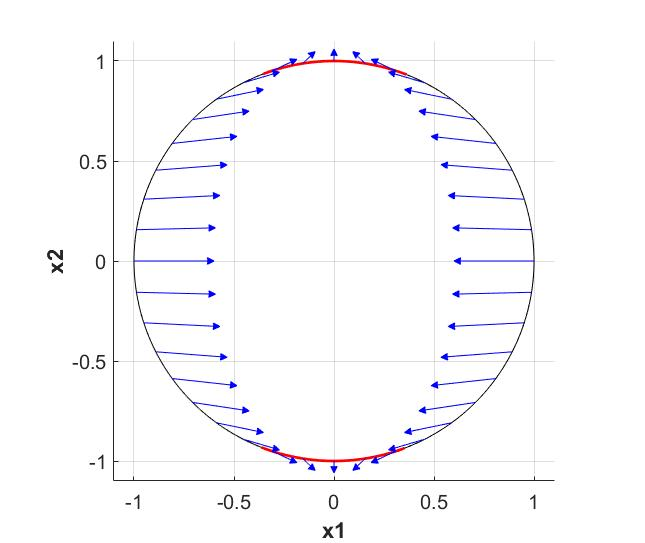
\includegraphics[scale=0.40]{ex1.jpg}
\end{center}

Moreover, the size of this "violating set" can be arbitrarily small based on the magnitude of the unstable eigenvalue. 

In this paper, we take the first step to close this gap. Since the identification and stability analysis of linear systems are well understood, we do so by focusing on switched linear systems. Note that identification and deciding the stability of arbitrary switched linear systems is NP-hard \cite{jungersBook}. Aside from their theoretical value, switched systems model the behavior of dynamical systems in the presence of known or unknown varying parameters. These parameters can model internal properties of the dynamical system such as uncertainties, look-up tables, values in a discrete register as well as exogenous inputs provided by a controller in a closed-loop control system. \textcolor{red}{Need to make these examples more specific.}

The stability of switched systems closely is closely related to the \emph{joint spectral radius} (JSR) of the matrices appearing in \eqref{eq:switchedSystem}. Under certain conditions deciding stability amounts to deciding whether JSR is less than one \cite{jungersBook}. In this paper, we present an algorithm to bound the JSR of a switched linear system from $N$ observations. This algorithm is based on tools from the random convex optimization literature \cite{campi}, and provides an upper bound on the JSR with a user-defined confidence level. As $N$ increases, this bound gets tighter. Moreover, with a closed form expression, we characterize what the exact trade-off between the tightness of this bound and the number of samples is. In order to understand the quality of our upper bound, the algorithm also provides a deterministic lower bound.

The organization of the paper is as follows: \textcolor{red}{TO BE FILLED.}
%. Topcu et.al. \cite{topcu}, Kapinski et.al. \cite{kapinski}construct Lyapunov function candidates using the simulation traces, however to be able to formally verify the constructed Lyapunov function, they require the knowledge of the full dynamics. In \cite{lazar} and \cite{lazar2} Bobiti and Lazar address this and provide sampling based probabilistic and deterministic guarantees of a given Lyapunov function candidate.

% The answer is immediate when \eqref{eq:dynamicalsystemGeneral} is a linear time-invariant system because we can simply identify $f$ by $n$ linearly independent output trajectories.  



%In this paper, we seek the answer to this question for switched linear systems for which the problem immediately becomes nontrivial. A switched linear systems is in the form:
%\begin{equation}\label{eq:switchedSystem}x_{k+1} = A_{\sigma(k)}x_k,\end{equation}
%where, $\sigma: \N \to \{1,2, \ldots, m\}$ is the switching sequence and $A_{\sigma(k)} \in \calM$, for all $\sigma$ and $k$. Aside from their theoretical value, switched systems model the behavior of dynamical systems in the presence of known or unknown varying parameters. These parameters can model internal properties of the dynamical system such as uncertainties, look-up tables, values in a discrete register as well as exogenous inputs provided by a controller in a closed-loop control system. 

%\textcolor{red}{There is no model.
%System are getting more complex, multimodal, lookup tables, thermodynamics, there is a need to ?prove properties about these systems, despite the fact that the modesl are mo complex are partially knowni Subcomponetns come from  different companies and black box.
%We still need to prove properties.
%The most important property in terms of control: stability.
%Even in the case when we have a model the stability is hard, for example Raphael, therefore we shouldn't expect we are gonna do better. The first step towards just based on switched systems. Because these are the very simple class of systems, resoanable it captures many applications.
%Even in the case of linear systems we cannot say anything. Here, we put the example where even the system is linear, we cannot say anything by just looking at the lyapunov functions decrease.}


%To make our reasoning clearer, we introduce the \emph{Lyapunov exponent} of the system \eqref{eq:switchedSystem}, which is a numerical quantity describing its stability.
%\begin{definition} Given a dynamical system as in \eqref{eq:dynamicalsystem} its \emph{Lyapunov exponent} is given by
%$$\rho =\inf{\{r:\,\forall x_0, \exists C\in \re^+: \quad x(0)=x_0 \Rightarrow x(t)\leq Cr^t\}}. $$
%\end{definition}
%Under certain conditions, deciding stability amounts to decide whether $\rho<1.$  In order to understand the quality of our techniques, we will actually try to prove lower and upper bounds on $\rho.$ 
%Assessing the stability of nonlinear systems by leveraging simulations has been an active area of research in the recent years. Simulation data has been used in both construction and verification of Lyapunov functions. Topcu et.al. \cite{topcu} and Kapinski et.al. \cite{kapinski} construct Lyapunov function candidates using the simulation traces, however to be able to formally verify the constructed Lyapunov function, they require the knowledge of the full dynamics. In \cite{lazar} and \cite{lazar2} Bobiti and Lazar address this and provide sampling based probabilistic and deterministic guarantees of a given Lyapunov function candidate. The presented method requires the knowledge of how fast the output of the system can change as the initial condition changes, and moreover the number of required samples increases exponentially in the dimension of the state, $n$.

%The stability of switched systems closely relates closely to the \emph{joint spectral radius} (JSR) of the matrices appearing in \eqref{eq:switchedSystem}. Under certain conditions deciding stability amounts to deciding whether JSR less than one or not. There has been a lot of work on developing algorithms to approximate this quantity, when the matrices appearing in \eqref{eq:switchedSystem} are known. Therefore, our work is also connected to the identification of switched systems, since once the system \eqref{eq:switchedSystem} is identified one can then apply these well-established results. However, there are two main reasons behind our quest to directly work on input-output pairs and bypassing the identification phase: (1) Even when $\calM$ is known, approximating the JSR is NP-hard \cite{jungers}. (2) Identifying the set $\calM$ is also NP-hard. Therefore, the existing identification techniques can identify $\calM$ up to an approximation error. As a result, how to relate this identification error to an error on the stability of \eqref{eq:switchedSystem} is still nontrivial.

%In this paper, we present an algorithm to approximate the JSR of a switched linear system from $N$ input-output pairs. This algorithm provides an upper bound on the JSR with a user-defined confidence level. As the number of samples increases, this bound gets tight. Moreover, we characterize with a closed form expression what the exact trade-off between the tightness of this bound and the number of samples is. In order to understand the quality of our technique, the algorithm also provides a deterministic lower-bound.

%The organization of the paper is follows: Section \label{preliminaries} introduces our notation and definitions from the switched linear system literature to present our results, Section \label{problemDefinition} formalizes the problem definition, Section \label{upperBound} provides an algorithm to compute a deterministic lower bound and 
%
%In this paper, we consider discrete-time switched linear systems of the form:
%\begin{equation}\label{eq:dynamicalsystem}x_{k+1} = A_{\sigma(k)}x_k,
%\end{equation}
%where, $x_k \in \R^n$, k is index of time and $\sigma: \N \to \{1,2, \ldots, m\}$ is the switching sequence. Let $y_k := x_{k+1}$. 
%We ask the following question:
%\begin{centering}
%\emph{Given N input-output-matrix pairs, $(x_1, y_1)$, $(x_2, y_2)$, $\ldots$, $(x_N, y_N)$ such that
%\begin{equation}\label{eq:triples}y_{k} = A_{\sigma(k)}x_k,
%\end{equation} for some $\sigma(k),$ what can we say about the stability of the system \eqref{eq:dynamicalsystem}?
%\end{centering}
%The only instance where answer to this question has been clearly shown is for linear time-invariant systems.
%
%Note that if \eqref{eq:dynamicalsystem} is a linear time-invariant system with only one mode, this question is easily answered by observing $n$ linearly independent data points. Switched systems can be used to model the behavior of a system of interest for different values of a parameter that varies. This parameter can represent internal parameters such as model uncertainties, as well as exogenous parameters such as inputs provided by a controller in a closed-loop control system. 


%- Stability analysis of dynamical systems is a challenging task. \\
%- Most methods in literature rely on knowing the model. Cite \\
%- How to make the case about the assumption of switched linear yet, we don't construct a model? Here cite
%something that says that this is a hard problem in general. (What is the relationship between switching linear regression)
%- Here we present stability analysis from data, this is easy for linear systems. We present something for switch linear.



%I can refer to the condition number paper?
\end{section}

\begin{section}{Preliminaries}
\label{sec:preliminaries}
\begin{subsection}{Notation}
% !TEX root = main.tex
We consider the usual finite normed vector space $(\R^n,\ell_2)$, $n \in \mathbb{N}_{> 0}$, with $\ell_2$ the classical Euclidean norm. We denote the set of linear functions in $\R^n$ by $\mathcal{L}(\mathbb{R}^n)$, and the set of real symmetric matrices of size $n$ by $\calS^n$. In particular, the set of positive definite matrices, which are matrices $P \in \calS^n$ such that $\forall\ x \in \R^n \setminus \{0\}$, $x^TPx > 0$, is denoted by $\calS^n_{++}$. We write $P \succ 0$ to state that $P$ is positive definite. Given a set $X \subset \R^n$, and $r \in \R_{> 0}$ we write \mbox{$rX := \{x \in X : rx\}$} to denote the scaling of this set. We denote by $\ball$ (respectively $\sphere$) the ball (respectively sphere) of unit radius centered at the origin.  We denote the ellipsoid described by the matrix $P \in \calS^n_{++}$ as $E_P$, i.e., $E_P:= \{x \in \R^n: x^TPx = 1\}$, and we denote by $\tilde{E}_P$ the volume in $\R^n$ defined by $E_P$: $\tilde{E}_P = \{x \in \R^n: x^TPx \leq 1\}$. We denote the spherical projector on $\sphere$ by $\proj_{\sphere}$. %We denote the homothety of ratio $r$ by $\calH_{r}$. 
%We denote by $\wp(M)$ the power set of $M$.

%We denote by $M$ the set $\{1,2,\dots,m\}$, ($m \in \N_{>0}$) and consider a switched linear system of modes $\calM = \{A_1, A_2,\dots, A_m\} \subset \R^{n \times n}$ indexed by $M$. We observe the system: 
%\begin{equation}\label{eq:dynamicalsystem}x_{k+1} = A_{\sigma(k)}x_k,
%\end{equation}
%where, $x_k \in \R^n$, k is index of time and $\sigma: \N \to M$ is the switching sequence. Let $y_k := x_{k+1}$. 
%We assume that we only know the number of modes $m$, the input $x_k$ and the output $y_k$ at each time $k$. We ignore what are the matrices and the index of the matrix which is applied at every time. We consider the following problem.

For an ellipsoid centered at the origin, and for any of its subsets $\calA$, the \emph{sector} defined by $\calA$ is the subset $$\{t \calA, \ t \in [0,1]\} \subset\ \R^n.$$ A sector induced by $\calA \subset E_P$ will be denoted by $E_P^{\calA}$. In the particular case of the unit sphere, we instead write $S^{\calA}$.

We consider in this work the classical unsigned and finite uniform spherical measure on $\sphere$, denoted by $\sigma^{n-1}$. It is associated to $\mathcal{B}_{\sphere}$, the spherical Borelian $\sigma$-algebra, and is derived from the Lebesgue measure $\lambda$. We have $\mathcal{B}_{\sphere}$ defined by $\calA \in \mathcal{B}_{\sphere}$ if and only if $S^{\calA} \in \mathcal{B}_{\mathbb{R}^n}$. The spherical measure $\sigma^{n-1}$ is defined by
$$\forall\ \calA \in \mathcal{B}_{\sphere},\, \sigma(\calA) = \frac{\lambda(S^{\calA})}{\lambda(B)}. $$
In other words, the spherical measure of a subset of the sphere is related to the Lebesgue measure of the sector of the unit ball it induces. Notice that $\sigma^{n-1}(\sphere) = 1$.
Since $P \in \calS_{++}^n$, it can be written in its Choleski form $P = UDU^{-1}$, where $D$ is the diagonal matrix of its eigenvalues and $U$ is an orthogonal matrix \cite{boyd}. Let \begin{equation}\label{choleski}L:=UD^{1/2}U^{-1}.\end{equation} Note that, $L^{-1}$ maps the elements of $\sphere$ to $E_P$. Then, we define the measure on the ellipsoid $\sigma_P$ on the $\sigma$-algebra $\mathcal{B}_{E_P}:=L^{-1}\mathcal{B}_\sphere$, where $\forall\, \calA \in \mathcal{B}_{E_P},\, \sigma_P({\calA}) = \sigma^{n-1}(L\calA)$. 

%
%
%
%We now relate $\sigma^{n-1}(V_{\sphere})$ to $\sigma_P(E')$. Consider the transformation linear transformation $L \in \calL({\R^n})$ mapping $\sphere$ to $E_P$. Note that since $P \in \calS^n$, it can be written in its Choleski form $P = U D U^{-1}$, with $D$ diagonal matrix of its eigenvalues, and $U \in O_n$. Then, $L = P^{1/2}=U D^{1/2} U^{-1}$ where $D^{1/2}$ is the diagonal matrix comprised of square root of elements of $D$.


For $m \in \N_{>0}$, we denote by $M$ the set $M=\{1,2, \ldots,m \}$. Set $M$ is provided with the classical $\sigma$-algebra associated to the finite sets: $\Sigma_M = \wp(M)$, where $\wp(M)$ is the set of subsets of $M$. We consider the uniform measure $\mu_M$ on $(M, \Sigma_M)$. 

We define $Z = \sphere \times M$ as the Cartesian product of the unit sphere and $M$. We denote the product $\sigma$-algebra $\mathcal{B}_{\sphere} \bigotimes \Sigma_M$ generated by $\mathcal{B}_{\sphere}$ and $\Sigma_M$: $\Sigma = \sigma( \pi_{\sphere}^{-1}(\mathcal{B}_{\sphere}),  \pi_{M}^{-1}(\Sigma_M))$, where $\proj_{\sphere}:Z \to \sphere$ and $\proj_M: Z \to M$ are the standard projections. On this set, we define the product measure $\mu = \sigma^{n-1} \otimes \mu_M$. Note that, $\mu$ is a uniform measure on $Z$ and $\mu(Z)=1$.   
\end{subsection}
\begin{subsection}{Stability of Switched Linear Systems}\label{sec:stab}
 % !TEX root = main.tex
A switched linear system related to a set of modes $\mathcal{M}= \{A_i, i \in M \}$ is of the form:
\begin{equation}\label{eq:switchedSystem}x_{k+1} = A_{\tau(k)}x_k,\end{equation}
with switching sequence $\tau: \N \to M$. There are two important properties of linear switched systems that we exploit in this paper.
\begin{property}\label{property:homogeneity}
Let $\xi(x, k, \tau)$ denote the state of the system \eqref{eq:switchedSystem} at time $k$ starting from the initial condition $x$ and with switching sequence $\tau$. The dynamical system \eqref{eq:switchedSystem} is homogeneous:
$$\xi(\gamma x, k, \tau)= \gamma \xi(x, k, \tau). $$
\end{property}
\begin{property}\label{property:convpres}
The dynamics given in \eqref{eq:switchedSystem} is convexity-preserving, meaning that for any set of points $X \subset \R^n$ we have:
$$ f(\conv{X})\subset \conv\{f(X)\}. $$
\end{property}

We now introduce the \emph{Lyapunov exponent} of the system, which is a numerical quantity describing its stability.
\begin{definition}Given a dynamical system as in \eqref{eq:dynamicalsystemGeneral}, its \emph{Lyapunov exponent} is given by
$$\rho =\inf{\{r:\,\forall\, x_0, \exists\, C\in \re^+: \xi(x_0, k)\leq Cr^k\}}. $$
\end{definition}
%Under certain conditions, deciding stability amounts to decide whether $\rho<1.$  In order to understand the quality of our techniques, we will actually try to prove lower and upper bounds on $\rho.$ 
%\textcolor{red}{@Raphael: We need  a theorem about the stability and $\rho<1$ here.}
%Under certain conditions deciding stability amounts to decide whether $\rho<1.$ 

In the case of switched linear systems, the Lyapunov exponent is known as the joint spectral radius of the set of matrices, which can be alternatively defined as follows:
\begin{definition} \cite{jungers_lncis} Given a set of matrices $\cM \subset \re^{n\times n},$ its \emph{joint spectral radius} (JSR) is given by
$$\rho(\cM) =\lim_{k\rightarrow \infty} \max_{i_1,\dots, i_k}\{||A_{i_1} \dots A_{i_k}||^{1/k}: A_{i_j}\in\cM\}. $$
\end{definition}

\begin{property}
[to cite: the Bible, corollary 1.1]
For any bounded set of matrices $\mathcal{M}$, the corresponding switched dynamical system is stable if and only if $\rho(\mathcal{M})<1$.
\end{property}

\begin{property}\label{rem:scaling}
[to cite: the bible, proposition 1.3]
For any bounded set of matrices $\mathcal{M}$, and any invertible matrix $T$, 
$$\rho(\mathcal{M})=\rho(T \mathcal{M} T^{-1}).$$
\end{property}

Note that this last result implies that the JSR is invariant under similarity transformations (and is a fortiori a homogeneous function: $\rho\left(\frac{\cM}{\gamma}\right)=\frac{\rho(\cM)}{\gamma}, \forall \gamma > 0$).

\end{subsection}
\begin{subsection}{Problem Formulation}
 % !TEX root = main.tex
We now formally present the problem we will be considering from now. We recall that our observations are traces of the form $(x_k,x_{k+1},\dots,x_{k+l})$ for some arbitrary $l \in \mathbb{N}_{>0}$, and that we do not have access to the mode applied to the system at each time step. 

To generate these traces, we assume that we can randomly pick a finite number of initial conditions $x_0^i \in \mathbb{R}^n$, and that a random sequence of $l$ modes is applied to each of these points. Hence, the probability event corresponding to a given observed trace $(x_k,x_{k+1},\dots,x_{k+l})$ is another $(l+1)$-tuple $(x_k,j_1,\dots,j_l)$. More precisely, we assume that we can uniformly sample such $(l+1)$-tuples in $Z_l = \sphere \times M^l$, giving us a sample denoted by 
\begin{equation*}
\begin{aligned}
\omega_N := & \{(x_0^1, j_{1,1}, \dots, j_{1,l}), (x_0^2, j_{2,1}, \dots, j_{2,l}), \ldots,\\
           & \qquad \qquad \qquad \qquad (x_0^N, j_{N,1},\dots, j_{N,l})\} \subset Z_l.
\end{aligned}
\end{equation*}
By uniformly sampling, we mean that the points in $\omega_N$ are drawn according to the measure $\mu_l$, i.e., the points $x_0^i$ are drawn from $\sphere$ according to the classical spherical measure $\sigma^{n-1}$, and the modes are drawn from $M$ according to the classical uniform measure $\mu_M$ at each time step. The space of sampling for the initial conditions is restricted to $\sphere$ since, as we recall, by Property \ref{property:homogeneity}, the system is homogeneous. 
\begin{rem}
Let us motivate the choice of considering a uniform sampling for the modes. Since we assume that we only have random observations of the state of the system, we do not know the process that generates this state: in particular, we ignore the process that picks the modes at each time step. We model this process with a random distribution. Here, we make the assumption that with nonzero probability, each mode is active. The problem would indeed not make a lot of sense otherwise, since in a such case, with probability $1$, the system would be unidentifiable and would prevent to ever observe some of its possible behaviors. By default, we take this distribution uniform since we cannot say that some modes are privileged a priori. But we can still take any other distribution satisfying our assumption; if we have a lower bound on the probability of each mode that is strictly positive, our guarantees naturally extend to them.
\end{rem}
From a sample $\omega_N$, we obtain the set of corresponding available observations 
\begin{equation}
\begin{aligned}
W_{\omega_N} := & \{(x_0^1,x_1^1, \dots, x_l^1), (x_0^2,x_1^2, \dots, x_l^2), \ldots,\\ 
& \qquad \qquad \qquad \qquad(x_0^N,x_1^N, \dots, x_l^N)\},
\end{aligned}
\end{equation}
which satisfy $$x_l^i= A_{j_{i,1}} \dots A_{j_{i,l}} x_0^i, \ \forall\ (x_0^i,x_1^i,\dots, x_l^i) \in W_{\omega_N}.$$
In this work, we aim at understanding what type of guarantees one can obtain on the stability of System \eqref{eq:switchedSystem} (that is, on the JSR of $\mathcal{M}$) from a finite, uniformly sampled, set of data. More precisely, we answer the following problem:
\begin{prob}\label{problem} 
Consider a finite set of matrices $\mathcal{M},$ describing a switched system \eqref{eq:switchedSystem}, and suppose that one has a set of $N$ observations $$\omega_N=\{(x_0^1, j_{1,1}, \dots, j_{1,l}), (x_0^2, j_{2,1}, \dots, j_{2,l}), \ldots, (x_0^N, j_{N,1},\dots, j_{N,l})\},$$ sampled according to the uniform measure $\mu_l$ on $Z_l$.
\begin{itemize}
\item For a given number $\beta \in (0,1)$, provide an upper bound $\overline{\rho(\omega_N)}$ on $\rho(\mathcal{M})$, together with a level of confidence $\beta$, that is, a number $\overline{\rho(\omega_N)}$ such that $$\mu_l \left( \{\omega_N: \ \rho(\mathcal{M}) \leq \overline{\rho(\omega_N)} \} \right) \geq \beta.$$
\item For the same given level of confidence $\beta$, provide a lower bound $\underline{\rho(\mathcal{M})}$ on $\rho(\mathcal{M})$.
\end{itemize}
\end{prob}
\begin{rem}
We will see in Section~\ref{sec:lowerBound} that a such level of confidence $\beta$ is not even required in the case of the lower bound. Indeed, we derive in Theorem~\ref{thm:lowerbound} a deterministic lower bound for a given (sufficiently high) number of observations. 
\end{rem}
The idea from now will be to leverage the fact that conditions for the existence of a CQLF for \eqref{eq:switchedSystem} can be obtained by considering a finite number of traces in $\mathbb{R}^n$ of the form $(x_k,x_{k+1}, \dots, x_{l})$. It will lead us to the following algorithm, that is the main result of our paper and that answers Problem~\ref{problem}:
%\begin{algorithm}
%\label{algo}
%\caption{Probabilistic upper bound}
\begin{alg}

\textbf{Input:} observations $W_{\omega_N}$ corresponding to a uniform random sample $\omega_N \subset Z$ of size $N \geq \frac{n(n+1)}{2}+1$;

\textbf{Input:} $\beta$ desired level of certainty;

\textbf{Compute:} $\gamma^{*}(\omega_N)$ optimal solution of Opt($\omega_N$), that we take as candidate for the upper bound;

\textbf{Compute:} $\varepsilon(\beta,\omega_N)$ the size of the of points where we might make the wrong inference on the upper bound;

\textbf{Compute:} $\delta(\varepsilon)$;

\textbf{Output:} $\frac{\gamma^{*}(\omega_N)}{\sqrt[2l]{n}} \leq \rho \leq \frac{\gamma^{*}(\omega_N)}{\sqrt[l]{\delta(\varepsilon)}}$, (upper bound valid with probability at least $\beta$ and $\delta(\beta, \omega_N)   \xrightarrow[N \to \infty]{} 1$).
%\end{algorithmic}
\end{alg}
%\end{algorithm}
\end{subsection}
\end{section}

\begin{section}{A Probabilistic Stability Guarantee}
\label{sec:upperbound}
% !TEX root = main.tex
In this section, we show that using Property \ref{property:homogeneity} and Property \ref{property:convpres}, by sampling finitely many points on a level set of a candidate CQLF, we can compute an upper bound on $\rho$. This section formalizes this discussion. Before proceeding to the main theorem, we motivate the upcoming technical discussion by stating the following theorem to which most of this section is devoted.

\begin{theorem} \label{thm:mainTheorem0} Let $\epsilon \in (0,1]$, $\beta \in [0,1)$. Consider a uniform random sampling of $\sphere \times M$, denoted by $\omega_N$. Let $\gamma^*$ and $P$ be the optimal solution to:
\begin{equation}\label{eqn:campiOpt01}
\begin{aligned}
& \text{min} & & \gamma \\
& \text{s.t.} 
&  & (A_j x)^TP(A_j x) \leq \gamma x^TPx,\,\forall (x, j) \in \omega_N \\
& && P \succ 0. \\
\end{aligned}
\end{equation}
Then for all $Z_P$ with $\sigma_P(Z_P)\leq \epsilon$, we have with probability at least $\beta$:
\begin{equation} \label{eqn:exceptEps}(A_j x)^TP(A_j x)\leq \gamma^*x^TPx,\,\forall\, x \in E_P \setminus Z_P, \forall j \in M.\end{equation}
Moreover, we can compute $\delta(\beta, \omega_N) < \infty$  such that:
\begin{equation}\label{eqn:contraction}E_{\delta^2P} \subset  \convhull (E_{P} \setminus Z_{P}),
\end{equation}
and $\lim_{N \to \infty} \delta(\beta, \omega_N) = 1.$
\end{theorem}

Once Theorem \ref{thm:mainTheorem0} is established, the main result of this section follows.

\begin{theorem}[Main Theorem] \label{thm:mainTheorem} Let $\omega_N$ be a uniform sampling of $\sphere \times M$, where $N \geq \frac{n(n+1)}{2}+1$ and $\beta \in [0,1)$. We can compute $\delta(\beta, \omega_N) < \infty$ such that with probability at least $\beta$ we have $$\rho \leq \frac{\gamma^*(\omega_N)}{\delta}.$$ Moreover, $\lim_{N \to \infty} \delta(\beta, \omega_N) = 1$.
\end{theorem}

%\begin{theorem}
%Consider a black-box switching system and $N$ samples of its dynamics as in \eqref{eq:switchedSystem}. Consider the optimal solution $(\lambda^*,P)$ which minimizes $\lambda$ in \eqref{eq:lowerbound}. For any factor $1<\delta,$ one can compute the level of confidence $\beta$ such that $\rho<\delta\cdot\lambda^*.$ 
%% denote $\gamma(P,\epsilon)$ the largest $\gamma$ such that $\gamma^2y_i^TPy_i\leq x_i^TPx_i$ 
%\end{theorem}
\begin{proof}Note that, by definition of $\gamma^*$ we have:
\begin{equation*} (A_j x)^TP(A_j x) \leq \gamma^* x^TPx, \quad \forall\, (x, j)  \in \omega_N \end{equation*}
for some $P \succ 0$. Then, by Theorem \ref{thm:mainTheorem0} we have:
\begin{equation*} (A_j x)^TP(A_j x) \leq \gamma^*x^TPx, \quad \forall\, x \in E_P \setminus Z_P,\, \forall j \in M, \end{equation*}
which can be rewritten as:
\begin{equation*}\frac{\calM}{\gamma^*}(E_P \setminus Z_P) \subseteq E_P \setminus Z_P.
\end{equation*}
By Property \ref{property:convpres}, this implies:
$$\frac{\calM}{\gamma^*} \conv(E_P \setminus Z_P) \subset \convhull(E_P \setminus Z_P).$$
Then, due to Theorem \ref{thm:mainTheorem0} we also have \eqref{eqn:contraction}, meaning:
$$\left(\frac{\cM}{\delta \gamma^*}\right) \convhull (E_P \setminus Z_P) \subset \convhull (E_P\setminus Z_P).$$
Then, $\delta\gamma^*$ is an upper bound on $\rho,$ with probability at least~$\beta$. 
\end{proof}

% !TEX root = main.tex

\begin{theorem}\label{thm:mainTheorem}Consider an $n$-dimensional switching system as in \eqref{eq:switchedSystem} and a uniform random sampling $\omega_N \subset Z$, where $N \geq \frac{n(n+1)}{2}+1$. Let $\gamma^*(\omega_N) $ be the optimal solution to \eqref{eqn:campiOpt01}. Then, for any given $\beta \in [0,1)$ and $\eta > 0$, we can compute $\delta(\beta, \omega_N)$, such that with probability at least $\beta$ we have:
$$\rho \leq \frac{\gamma^*(\omega_N) (1+ \eta)}{\delta(\beta, \omega_N)},$$
where $\lim_{N \to \infty}\delta(\beta, \omega_N) = 1$.
\end{theorem}

\begin{proof}
By definition of $\gamma^*(\omega_N)$ we have:
\begin{equation*} (A_j x)^TP(A_j x) \leq {(\gamma^*(1+\eta))}^2 x^TPx, \quad \forall\, (x, j)  \in \omega_N \end{equation*}
for some $P \succ 0$. 
Then, by rewriting Theorem \ref{mainTheorem0} we also have:
\begin{equation}\label{eqn:violation2}\mathbb{P}^N\left\{ \mu(V(\omega_N)) \leq \epsilon \right\} \geq 1- I(1-\epsilon; N-d, d+1),\end{equation}
where $I(\ell;a,b)$ is the regularized incomplete beta function. Let $\epsilon(\beta, N):=1- I^{-1}(1-\beta; N-d, d+1)$. 
Then, by Theorem \ref{mainTheorem0}, with probability at least $\beta$ the following holds:
\begin{equation*} (A_jx)^TP(A_jx) \leq  {(\gamma^*(1+\eta))}^2 x^TPx, \quad \forall (x, j) \in Z \setminus V.\end{equation*}
By Theorem \ref{thm:mainTheorem01}, this implies that with probability at least $\beta$ the following also holds:
\begin{equation*}(\bar{A_j} x)^T(\bar{A_j} x) \leq {\gamma}^2x^Tx,\,\, \forall\, x \in \sphere \setminus \sphere', \forall\, j \in M,\end{equation*}
for some $S'$ where $\sigma^{n-1}(S') \leq m\epsilon \kappa(P)$. Then, applying Lemma \ref{lemma:epsilon1}, we can compute
$$\delta(\beta, \omega_N) =\alpha(\epsilon'(\beta,N)),$$
where
\begin{equation}\label{eqn:eps2}\epsilon'(\beta, N) = \frac{1}{2} m\kappa(P)\epsilon(\beta,N)\end{equation} such that with probability at least $\beta$ we have:
\begin{equation*}
\bar{A_j} \ball \subset \frac{\gamma^*(\omega_N)(1+\eta)}{\delta(\beta, \omega_N)}\ball,\, \forall\, j \in M,
\end{equation*}
By Property \ref{rem:scaling}, this means that with probability at least $\beta$:
$$\rho \leq \frac{\gamma^*(\omega_N) (1 + \eta)}{\delta(\beta, \omega_N)},$$
which completes the proof of the first part of the theorem. The ratio $\frac{1}{2}$ introduced in the expression of $\epsilon'$ is due to the homogeneity of the system, which implies that $x \in V_{\sphere} \iff -x \in V_{sphere}$. We refer the interested reader to Appendix \ref{app:delta} for the second part of this proof, namely showing that $\lim_{N \to \infty}\delta(\beta, \omega_N) = 1$.



%
%$$\frac{\calM}{\gamma^*} \conv(E_P \setminus E') \subset \convhull(E_P \setminus E'),$$
%for some $E' \subset E_P$, where $\sigma_P(E') \leq \epsilon$.
%Then, due to Theorem \ref{thm:mainTheorem0} we also have \eqref{eqn:contraction}, meaning:
%$$\left(\frac{\cM}{\delta \gamma^*}\right) \convhull (E_P \setminus X_P) \subset \convhull (E_P\setminus X_P).$$
%Then, $\delta\gamma^*$ is an upper bound on $\rho,$ with probability at least~$\beta$. 
\end{proof}


\end{section}

%\begin{subsection}{Proving Theorem \ref{thm:mainTheorem0}}
%% !TEX root = main.tex

%\textcolor{red}{Here, we need to talk about proving the Lyapunov decrement in finitely, many points, talk about campi and then make a transition}

%In this section we suppose that we do not observe the modes, but only the pairs $(x_k,y_k).$
%The idea is that if we have an ellipsoid that is contracted for all our observed pairs $(x,y),$  it is not enough to imply stability, because we observed only some possible behaviours of the dynamics.  However, suppose that we observed that the $\lambda-$contraction of the polytope $\cP$ is satisfied for many values of $x,$ then, it is tempting to extrapolate our observation, and claim that (noting $y=f(x) $ as always),
Before proceeding to the proof of Theorem \ref{thm:mainTheorem0}, we introduce some further notation that will help us in the rest of this section. Let us consider $Z = \sphere \times M$, the Cartesian product of the unit sphere $\sphere$ with $M$. Every element of $Z$ can be written as $z = (x_z, j_z)$ with $x_z \in \sphere$ and $j_z \in M$. For notational simplicity, we drop the subscript $z$ whenever it is clear from the context. We define the classical projections of $Z$ on the sphere and $M$ by $\pi_{\sphere}: Z \to \sphere$ and $\pi_M: Z \to M$.

%The first statement in the Theorem \ref{thm:mainTheorem0} is equation \eqref{eqn:exceptEps}, which states that $\gamma^*$ and $P$ satisfying:
%\begin{equation*} (A_ix_i)^TP(A_ix_i)\leq \gamma^*x_i^TPx_i, \forall (x_i, A_i) \in \omega_N\end{equation*}
%also satisfies \eqref{eqn:exceptEps}. In other words, $\gamma^*$ and $P$ that are found from finitely many observations generalizes to the rest of the observations except a set of measure $\epsilon$. We now formalize.
To obtain an upper bound on $\rho$, the optimization problem we consider the following optimization problem:
\begin{equation}\label{eqn:campiOpt0}
\begin{aligned}
& \text{min} & & \gamma \\
& \text{s.t.} 
&  & (Ax)^TP(Ax) \leq \gamma x^TPx,\,\forall A \in \calM, \,\forall\, x \in \sphere,\\
& && P \succ 0. \\
\end{aligned}
\end{equation}
Note that if $P$ is a solution of \eqref{eqn:campiOpt0}, due to Property \ref{property:homogeneity}, then so is $\alpha P$ for any $\alpha \in \R_{> 0}.$ Therefore, the constraint $P \succ 0$ can be replaced with the constraint $P \succeq I$. Also note that, the optimal solution $\gamma^*$ satisfies $\rho \leq \gamma^*$. However, solving \eqref{eqn:campiOpt0} is hard since it involves infinitely many constraints. Therefore, for a given sampling $\omega_N$, we instead consider the optimization problem \eqref{eqn:campiOpt01} with finitely many constraints sampled from $Z$.

Let $\gamma^*(\omega_N)$ be the optimal solution of \eqref{eqn:campiOpt01}. We now analyze the relationship between the solutions of the optimization problem \eqref{eqn:campiOpt0} and:
\begin{equation}\label{eqn:campiOpt02}
\begin{aligned}
& \text{find} & & P \\
& \text{s.t.} 
&  & (A_j x)^TP(A_j x) \leq \gamma^* x^TPx,\,\forall (x, j) \in \omega_N \\
& && P \succ 0. \\
\end{aligned}
\end{equation}
We can rewrite \eqref{eqn:campiOpt02} in the following form:
\begin{equation}
\label{eqn:campiOpt2}
\begin{aligned}
& \text{find} & & P \\
& \text{s.t.} 
& & f_{\gamma^*}(P, z) \leq 0,\,\forall\ z \in Z\end{aligned}
\end{equation}
where $f_{\gamma^*}(P,z) = \max(f_1(P, z), f_2(P))$, and 
\begin{eqnarray*}
f_1(P, z) &:=& (A_j z)^TP(A_j z) - {\gamma^*}^2 x^TPx \\
f_2(P) &:=& \lambda_{\max}(-P) +1.
\end{eqnarray*}
We denote by  $\Opt(\omega_N)$ the optimization problem \eqref{eqn:campiOpt02} for the rest of the paper. Let $P(\omega_N)$ be the solution of $\Opt(\omega_N)$. We are interested in the probability of $P(\omega_N)$ violating at least one constraint in the original problem \eqref{eqn:campiOpt0}. Therefore, we define the constraint violation property next.

\begin{definition}(from \cite{campi}) The \emph{constraint violation probability} is defined as:
\begin{equation}\label{eqn:violation}
\calV^*(\omega_N)=
      \mathbb{P}\{z \in Z: f(P(\omega_N), z) > 0\},\, \forall\, \omega_N \in Z^{N*}\}.
\end{equation}
where $$Z^{N*}:=\{\omega_N \in Z^N: \text{the solution of $\Opt(\omega_N)$ exists}\}.$$ 
Due to the definition of $\gamma^*$, we know that a solution to $\Opt(\omega_N)$ exists for any $\omega_N$ and therefore $Z^{N*} = Z^N$. Also note that, since we have $\mathbb{P}(\calA) = \frac{\mu(\calA)}{\mu(Z)}$, we can rewrite \eqref{eqn:violation} as:
\begin{equation*}
\calV^*(\omega_N)=
      \frac{\mu(V)}{\mu(Z)},\, \forall\, \omega_N \in Z^N,
\end{equation*}
where $\mu$ is a measure on $Z$ and $V:=\{z \in Z: f(P(\omega_N), z) > 0\}$, i.e., the set of points for which at least one constraint is violated.
\end{definition}

The following theorem from \cite{campi} gives an explicit relationship between $\calV^*(\omega_N)$, $N$, and $n$.
\begin{theorem}[from \cite{campi}]\label{thm:campi}Let $d:=\frac{n(n+1)}{2}$. Consider the optimization problem $\Opt(\omega_N)$ given in \eqref{eqn:campiOpt02}. \textcolor{red}{How to talk about assumptions of this theorem here?} Then, for all $\epsilon \in (0,1)$ the following holds:
\begin{equation*}\mathbb{P}^N\{\{\calV^*(\omega) \leq \epsilon\} \} \geq 1- \sum_{j=0}^{d} \binom{N}{j}\epsilon^j (1-\epsilon)^{N-j}.\end{equation*}
\end{theorem}
Note that $\epsilon=1-I^{-1}(\beta, N-d, d+1)$, where $I$ is the regularized incomplete beta function. It can be interpreted as the ratio of the measure of points in $Z$ that might violate at least one of the constraints in \eqref{eqn:campiOpt02} to the measure of all points in $Z$.

%We now state our main theorem which gives a probabilistic upper bound on JSR, and devote the next section to proving it step by step.
%
%\begin{theorem}[Main Theorem] \label{thm:mainTheorem} For any $\eta > 0$, given $N \geq n+1$ and $\beta \in [0,1)$, we can compute $\delta(N) < \infty$ such that with probability at least $\beta$, $\rho \leq \frac{\gamma^*}{\delta}$. Moreover, $\lim_{N \to \infty} \delta(N) = 1$.
%\end{theorem}






%
%Note that, if such $P$ exists the optimal solution$\gamma^*$ satisfies $\rho \leq \gamma^*$. Also note that if $P$ is a solution to \eqref{eqn:campiOpt0}, due to Property \ref{property:homogeneity}, then so is $\alpha P$ for any $\alpha \in \R_{> 0}.$ Therefore, we the constraint $P \succ 0$ can be replaced with the constraint $P \succeq I$ and we can rewrite \eqref{eqn:campiOpt0} as in:
%\begin{equation}
%\label{eqn:campiOpt2}
%\begin{aligned}
%& \text{find} & & P \\
%& \text{s.t.} 
%& & f_\gamma(P, x) \leq 0,\,\forall A_i \in \calM, \,\forall\, s \in \sphere, \end{aligned}
%\end{equation}
%where $f_\gamma(P,x) = \max(f_1(P, x), f_2(P))$, and 
%\begin{eqnarray*}
%f_1(P, x) &:=& (A_ks)^TP(A_ks) - {\gamma^*}^2 s^TPs \\
%f_2(P) &:=& \lambda_{\max}(-P) +1.
%\end{eqnarray*}
%

%Note that if $P$ is a solution to \eqref{eq:lowerbound}, due to Property \ref{property:homogeneity}, then so is $\alpha P$ for any $\alpha \in \R_{> 0}.$ Therefore, we can rewrite the constraint $P \prec 0$ in \eqref{eq:lowerbound} as the following optimization problem:
%\begin{equation}
%\label{eqn:campiOpt1}
%\begin{aligned}
%& \min & & \gamma  \\
%& \text{s.t.} 
%&  & (A_ks)^TP(A_ks) \leq \gamma^2 s^TPs,\, \forall A_i \in \calM, \,\forall\, s \in \sphere,\\
%& & & P \succeq I.
%\end{aligned}
%\end{equation}


%
%
%
%We are interested in solving the following optimization problem for a given $\gamma \in (0,1)$:
%\begin{equation}
%\label{eqn:campiOpt0}
%\begin{aligned}
%& \text{find} & & P \\
%& \text{subject to} 
%&  & (A_is)^TP(A_is) \leq \gamma^2 s^TPs,\,\forall A_i \in \calM, \,\forall\, s \in \sphere,\\
%& && P \succ 0. \\
%\end{aligned}
%\end{equation}
%Note that, if such a $P$ exists, $\rho \leq \lambda$.


%\begin{equation}
%\label{eqn:campiOpt1}
%\begin{aligned}
%& \text{find} & & P \\
%& \text{subject to} 
%&  & (A_ks)^TP(A_ks) \leq \gamma^2 s^TPs,\, \forall A_i \in \calM, \,\forall\, s \in \sphere,\\
%& & & P \succeq I.
%\end{aligned}
%\end{equation}

%We define the linear isomorphism $\Phi$ as the natural mapping \mbox{$\Phi: \mathbb{R}^{\frac{n(n+1)}{2}} \to \mathbb{S}^n$.} Using this mapping, for a fixed $\gamma \in (0, 1]$ we can rewrite \eqref{eqn:campiOpt01} as the following convex optimization problem:
%
%\begin{equation}
%\label{eqn:campiOpt1}
%\begin{aligned}
%& \text{find} & & p \\
%& \text{subject to} 
%& & f(p,x) \leq 0, \forall x \in X.
%\end{aligned}
%\end{equation}
%where $f(p,x) = \max(f_1(p, x), f_2(p))$, and 
%\begin{eqnarray*}
%f_1(p,x) &:=& (A_ks)^T\Phi(p)(A_ks) - \gamma^2 s^T\Phi(p)s \\
%f_2(p) &:=& \lambda_{\max}(\Phi(-p)) +1.
%\end{eqnarray*}

%\textcolor{red}{We have to change the objective function!}
%$f(p, \xi)$ is defined as in:
%\begin{equation}\label{eqn:objFunction}f_\gamma(p, x) = \max\left((A_is)^T\Phi(p)(A_is) - \gamma x^T\Phi(p)x,\lambda_{\max}(\Phi(p)) - t, \lambda_{\max}(\Phi(-p)) +1\right).\end{equation}

%The optimization problem \eqref{eqn:campiOpt1} is convex in $p$.

%\begin{proof}The function $f_1(p,x)$ is clearly convex in $p$ for a fixed $x \in X$. The function 
%$\lambda_{max}: \mathbb{S}^n \to \R$ maps a symmetric positive matrix to its maximum eigenvalue. It is well-known that the function $\lambda_{\max}$ is a convex function of $P$. \cite{boyd}. This means that, $p \mapsto \Phi(\lambda_{\max}(p))$ is convex in $p$. Moreover, maximum of convex functions is also convex, which shows that $f(p, x)$ is convex in $p$.
%\end{proof}
%The optimization problem \eqref{eqn:campiOpt0} has infinitely many constraints. We next consider the following optimization problem where we sample $N$ constraints of \eqref{eqn:campiOpt0} independently and identically with the probability measure
%$\mathbb{P}(A) = \frac{\mu(A)}{\mu(X)}, \forall\, A \in \Sigma$, where $N \geq \frac{n(n+1)}{2}$, and $d := \frac{n(n+1)}{2}$. We denote this sampling by $\omega_N=\{x_1, x_2, \ldots, x_N\} \subset X$, and obtain the following convex optimization problem for a given $\gamma \in R$ $\Opt(\omega_N)$: 
%
%\begin{equation}
%\label{eqn:campiOpt2}
%\begin{aligned}
%& \text{find} & & P \\
%& \text{s.t.} 
%& & f_\gamma(P, x) \leq 0, \forall x \in \omega_N, \end{aligned}
%\end{equation}
%where $f_\gamma(P,x) = \max(f_1(P, x), f_2(P))$, and 
%\begin{eqnarray*}
%f_1(P, x) &:=& (A_ks)^TP(A_ks) - \gamma^2 s^TPs \\
%f_2(P) &:=& \lambda_{\max}(-P) +1.
%\end{eqnarray*}

%Let $P^*(\omega_N)$ be the solution of $\Opt(\omega_N)$. We are interested in the probability of $P^*(\omega_N)$ violating at least one constraint in the original problem \eqref{eqn:campiOpt0}. Therefore, we define constraint violation property next.



%We make the following assumptions on the problem $\Opt(\omega)$:
%\begin{enumerate}
%\item \label{assumption1} Uniqueness of solution: Note that this can be enforced by adding a tie-break rule of at most $\frac{n(n-1)}{2}$ convex conditions discriminating our solutions. 
%\item \label{assumption2} Nondegenaracy: with probability $1$, there is no redundancy in the constraint obtained from the sampling. 
%We can notice that a constraint obtained for a point $(s, k)$ gives us a constraint also on the point $(-s, k)$, and that a set of constraints containing some redundancy in them will be a set of constraints obtained from samples for a same mode. Now, let assume we consider for a fixed mode of index $k$ a nondegenerate sample of points $\{x_1, \dots, x_i\}$. Then if $x_{i+1} \notin \{(\pm s_{x_j},k), \ j \in \{1, \dots, i\} \}$ (which is a set of measure zero), the constraint obtained from $x_{i+1}$ is not redundant. Indeed, the mode of index $k$ might have all its eigenvalues but one with norm lower than $1$, and $x_{i+1}$ might be in the eigenspace of the latter eigenvalue (thus the constraint given by $x_{i+1}$ will be violated). Then, by considering the shortest distance between $x_{i+1}$ and the other points of the sample, we can choose for this eigenvalue a value close enough to $1$ (while being strictly greater than $1$) such that the constraints relative to the other points will still be satisfied.
%\end{enumerate}

%% !TEX root =main.tex

For a given sampling $\omega \in X^{N*}$, let $V:=\{x \in X: f(p^*(\omega),x) > 0\}$, i.e., the set of points for which at least one constraint is violated, and $V_\sphere, V_M$ be its projections on $\sphere$ and $M$, respectively. 

\begin{lemma}$\sigma^{n-1}(V_\sphere) \leq \frac{\mu(V)}{m_1}$, where $m_1 = \min \{\mu_M(\{k\}), k \in M\}$.\end{lemma}
\begin{proof}

Let $\calA \subset \Sigma$, $\calA_{\sphere} = \pi_{\sphere} (\calA)$ and $\calA_M = \pi_M (\calA)$. We notice that $\Sigma_M$ is the disjoint union of its $2^m$ elements $\{B_i, i \in \{1,2, \ldots 2^m\} \}$. Then $\calA$ is the disjoint union $\calA = \sqcup_{1 \leq i \leq 2^m} (\calA_i, B_i)$ where $\calA_i = \pi_M^{-1} (B_i) \in \sphere$. We notice that 
$\calA_{\sphere} = \sqcup_{1 \leq i \leq 2^m} \calA_i$, 
and
\begin{equation*}
\sigma^{n-1} (\calA_{\sphere}) = \sum_{1 \leq i \leq 2^m} \sigma^{n-1} (\calA_i).
\end{equation*}
We have 
\begin{eqnarray*}
\mu(\calA) = \mu(\sqcup_{1 \leq i \leq 2^m} (\calA_i, B_i)) &=& \sum_{1 \leq i \leq 2^m} \mu( (\calA_i, B_i)) \\
 &=& \sum_{1 \leq i \leq 2^m} \sigma^{n-1} \otimes \mu_M ((\calA_i, B_i)) \\
 & = &\sum_{1 \leq i \leq 2^m} \sigma^{n-1}(\calA_i) \mu_M (B_i).
\end{eqnarray*}
Let $m_1$ be the minimum value  of $\mu_M$ on its atoms: $m_1 = \min \{\mu_M(\{k\}), k \in M\}$ (recall that $m_1 > 0$). Then since $ \forall \ i$, $\mu_M(B_i) \geq m_1$, we have
\begin{equation}
\sigma^{n-1}(\calA_{\sphere}) \leq \frac{\mu(\calA)}{m_1}.
\end{equation}
This proves our statement by taking $\calA = V_{\sphere}$.
%Remark: In our case, we consider the special case where measures $\mu_1$ and $\mu_2$ are uniform and of total measure $1$ on $\sphere$ and $M$. $\mu_1$ is the classical spherical measure $\sigma^n$ and $\mu_2$ the classical uniform probability measure on $M$. We have then $m_2 = \frac{1}{m}$ and the inequality becomes:
\end{proof}

\begin{corollary} \label{cor:measure}When the modes are sampled from the set $M$ uniformly random, 
\begin{equation*}\sigma^{n-1}(V_\sphere) \leq m \mu(V). \end{equation*}
\end{corollary}

We consider the linear transformation mapping $\sphere$ to $E_P$, denoted by $L \in \mathcal{L}(\mathbb{R}^n)$. Note that since $P \in \calS^n(\R)$, it can be written in its Choleski form $P = U D U^{-1}$, with $D$ diagonal matrix of its eigenvalues, and $U \in O_n(\mathbb{R})$. We define $D^{1/2}$ the positive square root of $D$ as the matrix diag($\sqrt{d_1},\dots, \sqrt{d_n}$). Then, the positive square root of $P$ is $U D^{1/2} U^{-1}$. This means that, $L = P^{1/2}$. For the rest of the write-up, we denote $$V':=\proj_{\sphere}(L^{-1}(V_\sphere)),$$ and show how to upper bound $\sigma^{n-1}(V')$ in terms of $\mu(V)$.


Let us denote by $B_{V_{\sphere}}$ the sector of $\ball$ defined by $V_{\sphere}$. We recall the following result:

\begin{lemma} 
Let $\psi$ a smooth change of coordinates in $\mathbb{R}^n$ and $\cal{D} \subset \mathbb{R}^n$, whose image under $\psi$ is $\cal{D}' \subset \mathbb{R}^n$. We provide $\R^n$ with the classical Borel $\sigma$-algebra and the Lebesgue measure $\lambda$. Then
\begin{equation}
\lambda(\calD') = \int_{x \in \calD} 1_{x \in \calD} |\det J(\psi(x))| d\lambda(x),
\end{equation}
which becomes when $\psi \in \mathcal{L}(\R^n)$ (and thus $\forall\ x \in \R^n, \ \det J(\psi(x)) = \det(\psi)$ )
\begin{equation}
\lambda(\calD') = |\det(\psi)| \lambda(\calD).
\end{equation}
\end{lemma}


\begin{theorem} \label{lemma:lip}
\begin{equation}
\sigma^{n-1}(\proj_\sphere(L^{-1}(V_\sphere))) \leq \det(L^{-1}) \left(\frac{1}{\lambda_{\min}(L^{-1})}\right)^n \sigma^{n-1}(V_\sphere).
\end{equation}   
\end{theorem}

\begin{proof}
Let denote $C= L^{-1}(B_{V_{\sphere}})$. We have $\proj_{\sphere}(C) = V'$ and $B_{V'} \subset \calH_{\lambda_{\min}(L^{-1})}(C)$. 

We have then $\sigma^{n-1}(V') = \lambda(B_{V'}) \leq \lambda (\calH_{\lambda_{\min}(L^{-1})}(C))$.

Hence $\sigma^{n-1}(V') \leq \frac{1}{\lambda_{\min}(L^{-1})^n} \lambda(C)$.

By the former lemma, we have that $ \sigma^{n-1}(\proj_\sphere(L^{-1}(V_\sphere))) = \leq \det(L^{-1}) \left(\frac{1}{\lambda_{\min}(L^{-1})}\right)^n \sigma^{n-1}(V_\sphere)$.

%Note that the mapping $\proj_\sphere$ can be seen as the composition of the $\proj_{\sphere_r}$ for some $r > 0$, and $\calH_{\frac{1}{r}}$. Let $E':=L^{-1}(\sphere)$, then when $r < \min_{x \in E'}\|x\| = \lambda_{\min}(L^{-1})$ we have
%\begin{equation*}\proj_{\sphere_{\lambda_{\min}}} (x)= \proj_{\ball_{\lambda_{\min}}}(x) \qquad \forall\, x \in E'.
%\end{equation*}
%This shows that the restriction of $\proj_{\sphere_{\lambda_{\min}}}$ to $E'$ is a convex projector.

%We consider then $B_{\lambda_{\min}}$, and $P_{B_{\lambda_{\min}}}$ projector on $B_{\lambda_{\min}}$ defined in $\mathbb{R}^n$.

%Then by Corollary \ref{cor:proj} 
%\begin{equation}
%\lVert \proj_{\sphere_{\lambda_{\min}}}(x) - \proj_{\sphere_{\lambda_{\min}}}(y) \rVert \leq \lVert x - y \rVert, \qquad \forall \ x,y \in E'.
%\end{equation} 
%This shows that $1$ is a Lipschitz constant of the function $\proj_{\sphere_{\lambda_{\min}}}$ on $E'$. 

%By composing $\proj_{\sphere_{\lambda_{\min}}}$ with $\calH_{\frac{1}{\lambda_{\min}}}$, we obtain $\proj_\sphere$. Since the %Lipschitz constant of composition of two functions can be bounded by the multiplication of Lipschitz constants of each %function, the Lipschitz constant of $\Pi_S$ on $E'$ is $\frac{1}{\lambda_{\min}}$, which means that:
%\begin{equation}\label{eqn:lip}
%\lVert \proj_\sphere(x) - \proj_\sphere(y) \rVert \leq \frac{1}{\lambda_{\min}} \lVert x-y \rVert, \qquad \forall\,x,y \in E'.
%\end{equation}
%Note that, the inequality in \eqref{eqn:lip} is an equality when $x$ is in the eigenspace of $\lambda_{\min}$ and $y=-x$.

%Recall that for any smooth Lipschitz function $\phi$ with Lipschitz constant, Lip$(\phi)$, we have for all $x$, $|\det(J(\phi(x))| \leq \text{Lip}(\phi)^n$. Combining this with  \eqref{eqn:lip} and Lemma \ref{lemma:lip}, we get the statement %of the lemma.
\end{proof}

\begin{corollary}$\sigma^{n-1}(V') \leq m\epsilon \sqrt{\frac{\lambda_{\max}(P)^n}{\det(P)}}$,
where $\mu(V) = \epsilon$.
\end{corollary}



%% !TEX root = main.tex
We now show how to relate the upper bound on the measure of violating points $\sigma^{n-1}(V')$, with $\delta$. We do this by showing that the smallest $\delta$ is achieved when the violating points form a spherical cap of $\sphere$. We denote $\epsilon':=\frac{m\epsilon}{2} \sqrt{\frac{\lambda_{\max}(P)^n}{\det(P)}}$, where the additional factor $\frac{1}{2}$ follows from the homogeneity of the dynamics which implies a symmetry of $V_\sphere$, i.e., \begin{equation*}x \in V_{\sphere} \implies -x \in V_{\sphere}.\end{equation*}

Let $\dist$ be a distance on $\R^n$. The distance between a set $X \subset \R^n$ and a point $p \in \R^n$ is $\dist(X, p):=\inf_{x \in X}\dist(x,p)$. Note that the map $p \mapsto \dist(X,p)$ is continuous on $\R^n$.

\begin{definition}%[Spherical Cap]
We define the \emph{spherical cap} on $\sphere$ for a given hyperplane $c^Tx = k$ as:
\begin{equation*}\calC_{c,k} := \{x \in \sphere : c^Tx >k\}.\end{equation*}
\end{definition}

\begin{definition}A \emph{supporting hyperplane} of a set $X \subset \R^n$ is a hyperplane that has the following two properties:
\begin{itemize}
\item $X$ is entirely contained in one of the two closed half-spaces bounded by the hyperplane.
\item $X$ has at least one boundary-point on the hyperplane.
\end{itemize}
\end{definition}

\begin{remark}\label{suppHyperplaneRemark}\cite{boyd} Consider a convex set $X \subset \R^n$. For every $x \in \partial X$, there exists a supporting hyperplane containing $x$. Moreover, if $X$ is smooth, then this supporting hyperplane is unique.
\end{remark}
%\begin{proposition}Let $X \subset \R^n$ be a closed convex set. The set $X$ can be written as the intersection of all its support vectors:
%\begin{equation*} X = \cap_{i \in \partial X} c_i^Tx \leq k_i\end{equation*}
%\end{proposition}


%\begin{proposition}\label{distanceSet} Let $\dist$ be a distance on $\R^n$. The distance between a set $X \subset \R^n$ and a point $p \in \R^n$ is $\dist(X, p):=\inf_{x \in X}\dist(x,p)$. Then if $X$ is compact, we have:
%\begin{equation*}\dist(X,p)= \min_{x \in X}\dist(x,p). \end{equation*} 
%\end{proposition}

%\begin{proof}This is due to the fact that the function $\dist$ is continuous and hence attains its minimum on the compact set $X$.
%\end{proof}
\begin{remark}[see e.g. \cite{boyd}]\label{prop:distance}The distance between the point $x=0$ and the hyperplane $c^Tx = k$ is $\frac{|k|}{\|c\|}$.
\end{remark}

%\begin{lemma}\label{prop:distanceSet}Consider the boundary of the compact convex set
%\begin{equation*}X := \bigcap\limits_{i\in I}\{x: c_i^Tx \leq k_i\},\end{equation*} denoted by $\partial X$, then:
%\begin{equation*} \dist(\partial X,0) = \min_{i \in I} \frac{|k_i|}{\|c_i\|}.\end{equation*}
%\end{lemma}

%\begin{proof}Due to Proposition \ref{prop:distance} we have:
%\begin{equation}\dist(\partial X,0)= \inf_{i \in I} \dist\left(\{x: c_i^Tx = k_i\},0\right) = \inf_{i \in I}\koverc.
%\end{equation}
%Note that due to Proposition \ref{distanceSet}, the $\inf_{x \in \partial X}\dist(x,0)$ is attained by a point $x^* \in\partial X$ due to compactness of $\partial X$. Hence, there exists an $i \in I$ such that $c_i^Tx^*=k_i$ and this leads to: $\inf_{i \in I}\koverc = \min_{i \in I}\koverc$.
%\end{proof}

We now define the function $\Delta: \wp(\sphere) \to [0,1]$ as:
\begin{equation}\label{shrinkage}
\Delta(X) := \sup \{r: \ball_r \subset \conv(\sphere \setminus X)\}.\end{equation}
Note that, $\Delta(X)$ can be rewritten as:
\begin{equation}\label{shrinkage2}
\Delta(X) =  \dist(\partial  \conv(\sphere \setminus X), 0).
\end{equation}


\begin{lemma}\label{lemma:delta2}$\Delta(\calC_{c,k}) = \min\left(1, \frac{|k|}{\|c\|}\right)$.
\end{lemma}

\begin{proof}
Note that $$\conv(\sphere \setminus X)= \left\{x \in \ball : c^Tx \leq k \right\}.$$
\begin{eqnarray}
\nonumber \Delta(X) &=& \dist(\partial \conv(\sphere \setminus X), 0) \\
\nonumber &=& \min(\dist(\partial \ball, 0), \dist(\partial\{x : c^Tx \leq k\}, 0)) \\
\nonumber &=& \min(\dist(\sphere, 0), \dist(\{x : c^Tx = k\}, 0)) \\
\nonumber &=& \min\left(1, \frac{|k|}{\|c\|}\right).
\end{eqnarray}
\end{proof}
%\begin{lemma}\label{lemma:delta2}Given a set $X \subseteq \sphere$, let $\conv(\sphere \setminus X) := \ball \cap \calP$. Then we have:
%$$\Delta(X) = \min\left(\min_{i \in \partial X} \frac{|k_i|}{\|c_i\|}, 1\right),$$
%where $\left\{x \middle | c_i^Tx = k_i\right\} \in H_x(\calP)$ and $H \subseteq \{x : c_i^Tx \leq k_i\}$.
%\end{lemma}
%
%\begin{proof}
%Note that, $\calP = \cap_{i \in \partial X}\left\{x \middle | c_i^Tx \leq k_i\right\}$.
%\begin{eqnarray}
%\nonumber \Delta(X) &=& \sup \{r: \ball_r \subseteq \conv(\sphere \setminus X)\} \\
%\nonumber&=&\min \left(\dist(\partial \calP, 0), \dist(\sphere, 0) \right) \\
%\label{shrinkage1}&=&\min\left(\min_{i \in \partial X} \frac{|k_i|}{\|c_i\|},1\right) \qquad \qquad\text{due to Lemma\,} 
%{\ref{prop:distanceSet}}.
%\end{eqnarray}
%\end{proof}

\begin{corollary}\label{lemma:deltaMonotone}$\Delta(\calC_{c,k_1}) < \Delta(\calC_{c,k_2})$ when $k_1 < k_2$.
\end{corollary}

\begin{lemma}\label{lemma:muMonotone}$\sigma^{n-1}(\calC_{c,k_1}) < \sigma^{n-1}(\calC_{c,k_2})$, for $k_1 > k_2$.
\end{lemma}

\begin{proof}$\conv(\sphere \setminus \{x\in \sphere: c^Tx >k_1\}) \subset \conv(\sphere \setminus \{x\in \sphere: c^Tx >k_2\})$, for $k_1 > k_2$.
\end{proof}
Now we are ready to present the following lemma which is the key in proving that violating points forming a spherical cap leads to the worst case $\delta$.
\begin{lemma}\label{lemma:constructSC}For any set $X \subset \sphere$, there exist $c$ and $k$ such that $\calC_{c,k}$ satisfies:
\begin{equation*}\calC_{c,k} \subset X,
\end{equation*}
 and
\begin{equation}\Delta(\calC_{c,k}) = \Delta(X).
\end{equation}
\end{lemma}

\begin{proof} Let $\tilde{X} := \conv(S \setminus X)$.
Since $\dist$ is continuous and the set $\partial \tilde{X}$ is compact, there exists a point $x^* \in \partial \tilde{X}$, such that:
\begin{eqnarray}\nonumber \Delta(X) = \dist(\partial X_S, 0) = 
\label{deltaSupporting} \min_{x \in \partial \tilde{X}}\dist(x, 0) = \dist(x^*, 0).\end{eqnarray} 
Next, consider the supporting hyperplane of $\tilde{X}$ at $x^*$, which we denote by $\left\{x : c^Tx = k\right\}$. Note that this supporting hyperplane is a supporting hyperplane of the ball $\ball_{\Delta(X)}$ at $x^*$ since we have:
\begin{equation*} \partial \ball_{\Delta(X)} \subset \partial \tilde{X} \subset \left\{x : c^Tx = k\right\}.\end{equation*}  By Remark \ref{suppHyperplaneRemark}, this implies that $\left\{x : c^Tx = k\right\}$ is in fact the unique supporting hyperplane at $x^*$.
Then we have:
\begin{equation*}\Delta(X) =  \dist(x^*, 0) = \dist(\{x : c^Tx = k\}, 0) = \min\left(1, \frac{|k|}{\|c\|}\right).
\end{equation*}
Now, consider the spherical cap $\calC_{c,k}$. Then, by Lemma \ref{lemma:delta2} we have
$\Delta(\calC_{c,k}) =  \min\left(1, \frac{|k|}{\|c\|}\right)$. Therefore, $\Delta(X) = \Delta(\calC_{c,k})$.


We next show $\calC_{c, k} \subset X$. We prove this by contradiction. Assume $x \in \calC_{c,k}$ and $x \notin X$. Note that, if $x \notin X$, then $x \in \sphere \setminus X \subset \conv(\sphere \setminus X).$ Since $x \in \calC_{c,k}$, we have $c^Tx>k$. But due to the fact that $x \in \conv(\sphere \setminus X)$, we also have $c^Tx \leq k$, which leads to a contradiction. Therefore, $\calC_{c, k} \subset X$. 
\end{proof}
%\begin{lemma} The function $\tilde{\lambda}_{max} : \R^{n(n-1)/2} \to \R$ is convex in $z$.
%\end{lemma}

%\begin{proof}Let the function $\phi: \mathbb{S}^{n} \to \R^{n(n-1)/2}$ map a given symmetric matrix to a vector of its elements. Then we have $\tilde{\lambda}_{max}(z) = \lambda_{max}(\phi^{-1}(z))$. Note that the function $\phi$, and so is its inverse $\phi^{-1}$, and so is the maximum eigenvalue function. Since the composition a convex function with a linear function is convex, $\tilde{\lambda}_{max}$ is a convex function of $z$.
%\end{proof}


%\begin{section}{Main Results}
%
%\begin{lemma}If I lose $\epsilon$ measure on the product, I lose $m \epsilon$ points on $\sphere_1$.
%\end{lemma}
%
%\begin{proof}Let $X:=\sphere_1 \times M$ then $\sigma^{n-1}(bad) = \epsilon \sigma^{n-1}(\sphere_1 \times M) = \gamma \\
%\sigma^{n-1}(bad) = \sum_{x \in X} \sigma^{n-1}(bad \sphere_1) \leq \epsilon \sigma^{n-1}(X)$
%$\gamma = \sum_{x \in X} \sigma^{n-1}_1(x)\sigma^{n-1}_2(M_x)$
%We have $\sigma^{n-1}_2(M_x) \geq \sigma^{n-1}_2(m_i) = k > 0$. \\
%$\gamma \geq \sum k \sigma^{n-1}_1(x)$.
%This means that $\sigma^{n-1}_1(B_x) \leq m \epsilon$.
%\end{proof}

%\begin{lemma}\label{lemma:Convex}The function
%\begin{equation}\label{funcDelta0}\Delta_\epsilon(X):=\sup \{d: \ball_d \subset \conv(\sphere_1 \setminus X), \sigma^{n-1}(X) = \epsilon, X \subset \sphere_1\},
%\end{equation}
%attains its minimum when $X$ is a convex set.
%\end{lemma}
%\substack{\text{Some long text that} \\ \text{should be multiline}}
We now prove our main result.
\begin{theorem}\label{thm:mainSphericalCap}Let $\calX_{\epsilon'} = \{X \subset \sphere: \sigma^{n-1}(X) = \epsilon'\}$. Then, for any $\epsilon' \in (0,1)$, the function $\Delta(X)$ attains its minimum over $X_{\epsilon'}$ for some $X$ which is a spherical cap.
\end{theorem}

\begin{proof}We prove this via contradiction. Assume that there exists no spherical cap in $\calX_{\epsilon'}$ such that $\Delta(X)$ attains its minimum. This means there exists an $X^* \in \calX_{\epsilon'}$, where $X^*$ is not a spherical cap and $\argmin_{X \in \calX_{\epsilon'}}(\Delta(X))=X^*$. By Lemma \ref{lemma:constructSC}, we can construct a spherical cap $\calC_{c,k}$ such that $\calC_{c,k} \subset X^*$ and $\calC_{c,k} = \Delta(X^*)$. Note that, we further have $\calC_{c,k} \subsetneq X^*$, since $X^*$ is assumed not to be a spherical cap. This means that, there exists a spherical cap $\sigma^{n-1}(\calC_{c,k})$ such that $\sigma^{n-1}(\calC_{c,k}) < \epsilon'$. 

Then, the spherical cap $\calC_{c, \tilde{k}}$ with $\sigma^{n-1}(\calC_{c, \tilde{k}}) = \epsilon'$, satisfies $\tilde{k} < k$ due to Lemma \ref{lemma:muMonotone}. This implies $$\Delta(\calC_{c, \tilde{k}}) < \Delta(\calC_{c, k}) = \Delta(X^*)$$ due to Lemma \ref{lemma:deltaMonotone}. Therefore, $\Delta(\calC_{c, \tilde{k}}) < \Delta(X^*)$. This is a contradiction since we initially assumed that $\Delta(X)$ attains its minimum over $\calX_{\epsilon'}$ at $X^*$.
\end{proof}

\begin{corollary}\label{cor:main} Let $\beta \in (0,1)$. We have: $$\delta(\beta, \omega_N) =  \Delta(\calC_{c, k}),$$ where
$\sigma^{n-1}(\calC_{c,k}) = \epsilon'$.
\end{corollary}

\begin{theorem}Let $\beta \in (0,1)$. We have:
\begin{equation*}\delta(\beta, \omega_N) = \sqrt{(1-\alpha)}, \end{equation*}
where $\alpha := I^{-1}\left(\frac{\epsilon'\Gamma(\frac{d}{2})}{\pi^{d/2}}, \frac{d-1}{2}, \frac{1}{2}\right)$ and $$\Gamma(x)=\int_{0}^{\infty} t^{x-1} e^{-t} \text{d}t.$$ Here $I^{-1}$ is the inverse incomplete beta function, i.e.,  $I^{-1}(y, a,b)= x$ where $I_x(a,b)=y$.
\end{theorem}

\begin{proof}Let $h:=1-\delta = 1- \Delta(\calC_{c,k})$, where $\sigma^{n-1}(\calC_{c,k}) = \epsilon'$. It is well known \cite{sphericalCapRef} that the area of the spherical cap $\calC_{c,k} \subset \sphere$ is given by the equation:
\begin{equation}\sigma^{n-1}(\calC_{c,k}) = \frac{\pi^{d/2}}{\Gamma[\frac{d}{2}]}I_{2h-h^2} \left(\frac{d-1}{2}, \frac{1}{2}\right),
\end{equation}
where $I$ is the incomplete beta function. 
Since, \mbox{$\sigma^{n-1}(\calC_{c,k})=\epsilon'$,} we get the following set of equations:
\begin{eqnarray}\nonumber \frac{\epsilon' \Gamma[\frac{d}{2}]}{\pi^{d/2}} &=& I_{2h-h^2}\left(\frac{d-1}{2}, \frac{1}{2}\right) \\
\nonumber 2h-h^2 &=&  I^{-1}\left(\frac{\epsilon'\Gamma(\frac{d}{2})}{\pi^{d/2}}, \frac{d-1}{2}, \frac{1}{2}\right) \\
\nonumber 2h-h^2 & = & \alpha \\
\label{lasteqn}h^2 -2h +\alpha &=& 0.
\end{eqnarray}
From \eqref{lasteqn}, we get $h=1\pm \sqrt{(1-\alpha)}$. Since $h\leq1$, we conclude that \mbox{$\Delta(\calC_{c,k}) = \sqrt{(1-\alpha)}$.} Note that, $\Delta(\calC_{c,k})$ only depends on $\epsilon'$ for fixed $n$.
\end{proof}

\begin{corollary}\label{cor:final}Let $\beta \in (0,1)$. $$\lim_{N \to \infty} \delta(\beta, \omega_N) = 1.$$
\end{corollary}

\begin{proof} 
We first prove that $\lim_{N \to \infty} \epsilon(\beta, N)= 0$. Note that, we can upper bound $1-\beta$ as follows:
\begin{equation}\label{eqn:beta}1-\beta = \sum_{j=0}^d {{N}\choose{j}} \epsilon^j (1-\epsilon)^{N-j} \leq  (d+1)N^d (1-\epsilon)^{N-d}.
\end{equation}
We prove $\lim_{N \to \infty} \epsilon(\beta, N) = 0$ by contradiction. Assume that $\lim_{N \to \infty} \epsilon(\beta, N) \not= 0$. This means that, there exists some $\delta > 0$ such that $\epsilon(\beta, N) > \delta$ infinitely often. Then, consider the subsequence $N_k$ such that $\epsilon(\beta, N_k) > \delta$, $\forall\, k.$ Then, by \eqref{eqn:beta} we have:
\begin{equation*}1-\beta\leq (d+1)N_k^d (1-\epsilon)^{N_k-d} \leq (d+1)N_k^d (1-\delta)^{N_k-d}\, \forall\,k \in \N. 
\end{equation*}
Note that $\lim_{k \to \infty}(d+1)N_k^d (1-\delta)^{N_k-d} = 0.$ Therefore, there exists a $k'$ such that, we have $$(d+1)N_{k'}^d (1-\delta)^{N_k'-d} < 1 - \beta,$$ which is a contradiction. Therefore, we must have  $\lim_{N \to \infty} \epsilon (\beta, N) = 0$.

\textcolor{red}{Still to show: If $\frac{\lambda{\max}(P)}{\lambda{\min}(P)}$ is uniformly bounded in $N$, then
since $I^{-1}$ is monotonic in its first parameter, $\delta = \sqrt{1-\alpha}$ tends to $1$ as $\epsilon \to 0$.}
\end{proof}

Putting together Theorem \ref{thm:campi} with Corollary \ref{cor:main} and Corollary \ref{cor:final}, the result of Theorem \ref{thm:mainTheorem0} follows.

%\end{subsection}

\begin{section}{A Deterministic Lower Bound for the JSR}
\label{sec:lowerbound}
% !TEX root = main.tex
We start by proving the lower bound, which is based on the following theorem from the switched linear system literature.

\begin{theorem}\cite[Theorem 2.11]{jungers_lncis}\label{thm:john}
For any bounded set of matrices such that $\rho(\cM)<\frac{1}{\sqrt{n}},$ there exists a Common Quadratic Lyapunov Function (CQLF) for $\cM,$ that is, a $P\succ 0$ such that: $$\forall A\in \cM,\, A^TPA\preceq P. $$
\end{theorem}

The following theorem shows that the existence of a CQLF for \eqref{eq:switchedSystem} can be checked by collecting $N$ observation pairs.
%
%The existence of a CQLF for our (potentially scaled) blackbox system is certainly something we can check: after collecting $N$ observations, one can solve the following optimization problem efficiently. 
%

%Indeed, when $\lambda $ is fixed, the problem is a set of LMIs, and $\lambda $ can be optimized by bisection.

\begin{theorem}
For a given sampling: $$\omega_N = \{x_1, x_2, \ldots, x_N\},$$ let $\gamma^*(\omega_N)$ be the optimal solution of the following optimization problem:
\begin{eqnarray}
\nonumber \mbox{min}&&\gamma\\
 s.t.& & \label{eq:lowerbound}y_i^T P y_i \leq \gamma^2 x_i^TPx_i,\,  \forall \,i : \,1\leq i \leq N\\
\nonumber && P \succ 0.
\end{eqnarray}
If $\gamma^*(\omega_N)<\infty,$ we have:
$$\rho(\cM) \geq \frac{\gamma^*}{\sqrt{n}}.$$ Note that, \eqref{eq:lowerbound} can be solved by bisection on $\gamma$.

\end{theorem}
\begin{proof}
Using Remark \ref{rem:scaling}, for any $\epsilon > 0$, $\frac{\cM}{(\gamma^*-\epsilon),}$ has no CQLF. Then, applying Theorem \ref{thm:john} we get
\begin{equation*}\frac{\rho(\cM)}{\gamma^*} \geq \frac{1}{\sqrt{n}}.\end{equation*}
\end{proof}
\end{section}

\begin{section}{Experimental Results}
\label{sec:experiments}
% !TEX root =main.tex
We illustrate our technique on a two-dimensional switched system with $4$ modes. We fix the condifence level, \mbox{$\beta = 0.92$} and compute both upper and lower bounds on the JSR for $N:=15+50k,\, k \in\{0, \ldots, 10\}.$ We demonstrate the average performance of our algorithm over $10$ different runs in Figure \ref{fig:11} and Figure \ref{fig:21}. Figure \ref{fig:11} demonstrates the evolution of $\delta(\beta, N)$ as $N$ increases. We observe that $\delta$ converges to $1$ as expected. In Figure \ref{fig:21}, we plot the upper bound and lower bound for the JSR of the system computed by Theorem \ref{thm:mainTheorem} and Theorem \ref{thm:lowerbound}, respectively. To demonstrate the performance of our technique, we also provide the JSR approximated by the JSR toolbox \cite{jsrtoolbox}, which turns out to be $0.7727$. As can be seen, the upper bound approaches to a close vicinity of the real JSR with approximately 250 samples. In addition, the lower bound converges to $\frac{\rho}{\sqrt{n}}$ as expected.

\begin{figure}
\begin{center}
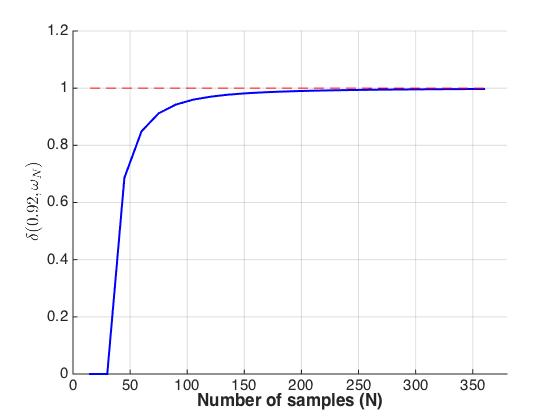
\includegraphics[scale=0.35]{delta1.jpg}

\caption{Evolution of $\delta$ along $N$.}
\label{fig:11}
\end{center}
\end{figure}

\begin{figure}
\begin{center}
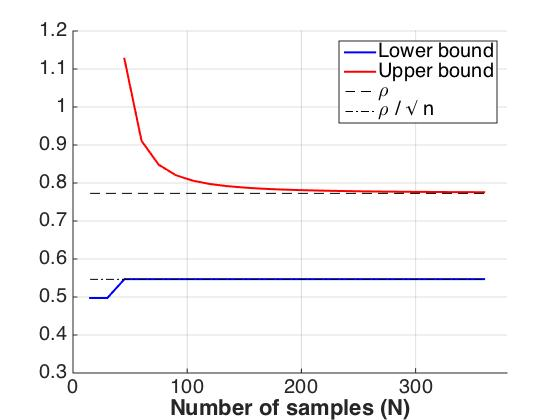
\includegraphics[scale=0.35]{bounds1.jpg}

\caption{Evolution of the bounds along $N$.}
\label{fig:21}
\end{center}
\end{figure}

We next test our algorithm with a $4$-dimensional system, with $5$ modes. We observe a slower convergence of $\delta$ as well as upper and lower bounds on $\rho$.
\textcolor{blue}{[to add plots here, but they are not super nice: we do not see the convergence to $1$ of $\delta$: even after $10 000$ points, $\delta$ is below $0.85$].}

Finally, we randomly generate $10,000$ cases with systems of dimension between $2$ and $7$, number of modes between $2$ and $5$, and size of samples $N$ between $30$ and $800$. We take $\beta = 0.92$ and we check if the upper bound computed by our techniques is greater than the actual JSR of the system. We get $xxx$ positive tests, out of $10,000$, which gives us a probability of $??$ of the correctness of the upper bound computed. Note that, this probability is significantly above the provided $\beta$. This is expected, since our techniques are based on worst-case analysis and thus conservative.




\end{section}

\begin{section}{Conclusions}
\label{sec:conclusions}
% !TEX root =main.tex
In this work, we have investigated the question of how one can conclude stability of a system, by only observing trajectories, without having any mathematical description of the dynamics ruling the system.   Our goal, motivated by both practical and theoretical considerations, was to avoid combining identification of the system with classical stability analysis techniques.  Indeed, in real-world applications, often the true equations describing the dynamics might be extremely complex or nonstandard, or might even not be well defined. Moreover, identification of such complex systems is typically hard, and it is not clear how observation or computation errors would propagate in such a two-step strategy. 

For these reasons, we aim at understanding how the observation of well-behaved trajectories \emph{intrinsically} implies stability of a system.  As argued in the introduction, it is easily seen that some standing assumption should be made on the system, in order to allow for any sort of nontrivial certificate, solely from a finite number of observations. The novelty of our contribution is twofold: 
First, we use as such a standing assumption that the system is a switching linear system.  This assumption covers a wide range of systems of interest nowadays, and to our knowledge no 'black-box stability' result was available so far on switching systems.  
Second, we apply powerful techniques from chance constrained optimization.  The application is not obvious, and relies on geometric properties of linear switching systems. We believe that this guarantee is quite powerful, in view of the hardness of the general problem, and in the future, we plan to investigate how to generalize it to more complex or realistic systems.  We are also improving the numerical properties of our technique by incorporating Sum-Of-Squares optimization, and relaxing the sampling assumptions on the observations.

\end{section}

\appendix
\label{appendix}
% !TEX root = main.tex
\begin{section}{Precisions on Measures Definitions}\label{app:measures}

For an ellipsoid centered at the origin, and for any of its subsets $\mathcal{A}$, the \emph{sector} defined by $\mathcal{A}$ is the subset $$\{t \mathcal{A}, \ t \in [0,1]\} \subset\ \mathbb{R}^n.$$ We denote by $E_P^{\mathcal{A}}$ the sector induced by $\mathcal{A} \subset E_P$. In the particular case of the unit sphere, we instead write $\sphere^{\mathcal{A}}$. We can notice that $E_P^{E_P}$ is the volume in $\mathbb{R}^n$ defined by $E_P$: $E_P^{E_P} = \{x \in \mathbb{R}^n: x^T P x \leq 1\}$.

The spherical Borelian $\sigma$-algebra, denoted by $\mathcal{B}_{\sphere}$, is defined by $$\mathcal{A} \in \mathcal{B}_{\sphere} \iff \sphere^{\mathcal{A}} \in \mathcal{B}_{\mathbb{R}^n}.$$ We provide $(\sphere,\mathcal{B}_{\sphere})$ with the classical, unsigned and finite uniform spherical measure $\sigma^{n-1}$ defined by
$$\forall\ \mathcal{A} \in \mathcal{B}_{\sphere},\, \sigma(\mathcal{A}) = \frac{\lambda(\sphere^{\mathcal{A}})}{\lambda(\ball)}. $$
In other words, the spherical measure of a subset of the sphere is related to the Lebesgue measure of the sector of the unit ball it induces. Notice that $\sigma^{n-1}(\sphere) = 1$.

Since $P \in \mathcal{S}_{++}^n$, we recall that it can be written in its Cholesky form \eqref{cholesky}. Note that, $L^{-1}$ maps the elements of $\sphere$ to $E_P$. Then, we define the measure on the ellipsoid $\sigma_P$ on the $\sigma$-algebra $\mathcal{B}_{E_P}:=L^{-1}(\mathcal{B}_\sphere)$, where $\forall\, \mathcal{A} \in \mathcal{B}_{E_P},\, \sigma_P({\mathcal{A}}) = \sigma^{n-1}(L\mathcal{A})$. 

Set $M$ is provided with the classical $\sigma$-algebra associated to the finite sets: $\Sigma_M = \wp(M)$, where $\wp(M)$ is the set of subsets of $M$. We provide $(M, \Sigma_M)$ with the uniform measure $\mu_M$. Similarly, we define $\Sigma_{M^l}$ as the product $\bigotimes^l \Sigma_M$ (which is here equal to $\wp(M)^l$), and we provide $(M^l, \Sigma_{M^l})$ with the uniform product measure $\mu_{M^l} = \otimes^l \mu_M$.

We can now denote the product $\sigma$-algebra $\mathcal{B}_{\sphere} \bigotimes (\Sigma_{M^l})$ generated by $\mathcal{B}_{\sphere}$ and $\Sigma_{M^l}$: $\Sigma = \sigma( \pi_{\sphere}^{-1}(\mathcal{B}_{\sphere}),  \pi_{M^l}^{-1}(\Sigma_{M^l}))$, where $\pi_{\sphere}: Z_l \to \sphere$ and $\pi_{M^l}: Z_l \to M^l$ are the standard projections. On $(Z_l,\mathcal{B}_{\sphere} \bigotimes (\Sigma_{M^l}) )$, we define the product measure $\mu_l = \sigma^{n-1} \otimes \mu_{M^l}$. Note that, $\mu_l$ is a uniform measure on $Z_l$ and $\mu_l(Z_l)=1$.  

\end{section}


\begin{section}{Proof of Corollary~\ref{cor:gettingRidOfm}}\label{proof:cor_m}
We prove here Corollary~\ref{cor:gettingRidOfm} stated in section~\ref{sec:IntroMainThm}.

Let $\sphere' = \pi_{\sphere}(V)$. We know that $\Sigma_{M^l}$ is the disjoint union of its $2^{m^l}$ elements $\{\mathcal{M}^l_i, i \in \{1,2, \dots, 2^{m^l} \} \}$. Then $V$ can be written as the disjoint union $V = \sqcup_{1 \leq i \leq 2^{m^l}} (\mathcal{S}_i, \mathcal{M}^l_i)$ where $\mathcal{S}_i \in \Sigma_{\sphere}$. We notice that 
$\sphere' = \sqcup_{1 \leq i \leq 2^{m^l}} \mathcal{S}_i$, 
and
\begin{equation*}
\sigma^{n-1} (\sphere') = \sum_{1 \leq i \leq 2^{m^l}} \sigma^{n-1} (\mathcal{S}_i).
\end{equation*}
We have 
\begin{eqnarray*}
\mu_l(V) &=& \mu_l \left( \sqcup_{1 \leq i \leq 2^{m^l}} (\mathcal{S}_i, \mathcal{M}^l_i) \right) = \sum_{1 \leq i \leq 2^{m^l}} \mu_l \left( \mathcal{S}_i, \mathcal{M}^l_i \right) \\
 &=& \sum_{1 \leq i \leq 2^{m^l}} \sigma^{n-1} \otimes \mu_{M^l} \left( \mathcal{S}_i, \mathcal{M}^l_i \right) \\
 &=& \sum_{1 \leq i \leq 2^{m^l}} \sigma^{n-1}(\mathcal{S}_i) \mu_{M^l} (\mathcal{M}^l_i).
\end{eqnarray*}

Note that we have $\min_{(j_1,\dots,j_l) \in M^l} \mu_{M^l}(\{j_1,\dots,j_l\}) = \frac{1}{m^l}.$ Then since $ \forall \ i$, $\mu_{M^l}(\mathcal{M}^l_i) \geq \min_{(j_1,\dots,j_l) \in M^l} \mu_{M^l}(\{j_1,\dots,j_l\}) = \frac{1}{m^l}$, we get:
\begin{equation}
\sigma^{n-1}(sphere') \leq \frac{\mu_l(V)}{\frac{1}{m^l}} \leq m^l \varepsilon.
\end{equation}
This means that 
\begin{equation}\label{eqn:P2}
\begin{aligned}
& (A_{j_l} A_{j_{l-1}} \dots A_{j_1} x)^T P (A_{j_l} A_{j_{l-1}} \dots A_{j_1} x) \leq \gamma^{2l} x^T P x,\\
& \qquad \qquad \qquad \qquad \forall\, x \in \sphere \setminus \sphere', \,\forall\, (j_1,\dots,j_l) \in M^l,
\end{aligned}
\end{equation}
where $\sigma^{n-1}(\sphere') \leq m^l \varepsilon.$

\end{section}


\begin{section}{Preliminary Results on Spherical Caps}\label{sec:app_prelim_caps}

Before proceeding to the proof of Proposition~\ref{lemma:propositionSphericalCaps}, we first introduce some necessary definitions and related background on spherical caps. We recall that a \emph{spherical cap} on $\sphere$ for a given hyperplane $c^Tx = k$ is defined by $\mathcal{C}_{c,k} := \{x \in \sphere : c^Tx >k\}$.


\begin{rem}\label{lemma:muMonotone}
Consider the spherical caps $\mathcal{C}_{c, k_1}$ and $\mathcal{C}_{c, k_2}$ such that $k_1 > k_2$, then we have:
$$\sigma^{n-1}(\mathcal{C}_{c,k_1}) < \sigma^{n-1}(\mathcal{C}_{c,k_2}).$$
\end{rem}


\begin{rem}\label{prop:distance}
The distance between the point $x=0$ and the hyperplane $c^Tx = k$ is $\frac{|k|}{\|c\|}$.
\end{rem}

We also recall that we defined in section~\ref{sec:pbsphere} the function $\Delta: \wp(\sphere) \to [0,1]$ as $\Delta(X) := \sup \{r: r\ball \subset \conv(\sphere \setminus X)\}$.


\begin{lem} \label{lemma:delta2} 
Consider the spherical cap $\mathcal{C}_{c,k}$. We have:
$$\Delta(\mathcal{C}_{c,k}) = \min\left(1, \frac{|k|}{\|c\|}\right).$$
\end{lem}

\begin{pf}
Note that: $$\conv(\sphere \setminus X)= \left\{x \in \ball : c^Tx \leq k \right\}.$$
Then the following equalities hold:
\begin{eqnarray}
\nonumber \Delta(X) &=& \dist(\partial \conv(\sphere \setminus X), 0) \\
\nonumber &=& \min(\dist(\partial \ball, 0), \dist(\partial\{x : c^Tx \leq k\}, 0)) \\
\nonumber &=& \min(\dist(\sphere, 0), \dist(\{x : c^Tx = k\}, 0)) \\
\nonumber &=& \min\left(1, \frac{|k|}{\|c\|}\right).
\end{eqnarray}
\end{pf}

\begin{cor}\label{lemma:deltaMonotone} 
Consider the spherical caps $\mathcal{C}_{c, k_1}$ and $\mathcal{C}_{c, k_2}$ such that $k_1 \leq k_2$. Then we have: $$\Delta(\mathcal{C}_{c,k_1}) \leq \Delta(\mathcal{C}_{c,k_2}).$$
\end{cor}

\begin{lem}\label{lemma:constructSC}
For any set $X \subset \sphere$, there exist $c$ and $k$ such that $\mathcal{C}_{c,k}$ satisfies: $\mathcal{C}_{c,k} \subset X,$ and $\Delta(\mathcal{C}_{c,k}) = \Delta(X).$
\end{lem}

\begin{pf} Let $\tilde{X} := \conv(S \setminus X)$.
Since $\dist$ is continuous and the set $\partial \tilde{X}$ is compact, there exists a point $x^* \in \partial \tilde{X}$, such that:
\begin{eqnarray}\nonumber \Delta(X) = \dist(\partial\tilde{X}, 0) = 
\label{deltaSupporting} \min_{x \in \partial \tilde{X}}\dist(x, 0) = \dist(x^*, 0).\end{eqnarray} 
Next, consider the hyperplane which is tangent to the ball $\Delta(X)\ball$ at $x^*$, which we denote by $\left\{x : c^Tx = k\right\}$.
%\begin{equation*} \partial (\Delta(X)\ball) \subset \tilde{X} \subset \left\{x : c^Tx \leq k\right\}.\end{equation*}  By Remark \ref{suppHyperplaneRemark}, this implies that $\left\{x : c^Tx = k\right\}$ is in fact the unique supporting hyperplane at $x^*$.
Then we have:
\begin{equation*}\Delta(X) =  \dist(x^*, 0) = \dist(\{x : c^Tx = k\}, 0) = \min\left(1, \frac{|k|}{\|c\|}\right).
\end{equation*}
Now, consider the spherical cap defined by this tangent plane i.e., $\mathcal{C}_{c, k}$. Then, by Lemma \ref{lemma:delta2} we have
$\Delta(\mathcal{C}_{c,k}) =  \min\left(1, \frac{|k|}{\|c\|}\right)$. Therefore, $\Delta(X) = \Delta(\mathcal{C}_{c,k})$.


We next show $\mathcal{C}_{c, k} \subset X$. We prove this by contradiction. Assume $x \in \mathcal{C}_{c,k}$ and $x \notin X$. Note that, if $x \notin X$, then $x \in \sphere \setminus X \subset \conv(\sphere \setminus X).$ Since $x \in \mathcal{C}_{c,k}$, we have $c^Tx>k$. But due to the fact that $x \in \conv(\sphere \setminus X)$, we also have $c^Tx \leq k$, which leads to a contradiction. Therefore, $\mathcal{C}_{c, k} \subset X$. 
\end{pf}

We are now able to prove Proposition~\ref{thm:mainSphericalCap} given in section~\ref{sec:pbsphere}, which states that, for any $\varepsilon \in (0,1)$, the function $\Delta(X)$ attains its minimum over $\mathcal{X}_{\varepsilon}$ for some $X$ which is a spherical cap.


\begin{pf}
We prove this via contradiction. Assume that there exists no spherical cap in $\mathcal{X}_{\varepsilon}$ such that $\Delta(X)$ attains its minimum. This means there exists an $X^* \in \mathcal{X}_{\varepsilon}$, where $X^*$ is not a spherical cap and $\argmin_{X \in \mathcal{X}_{\varepsilon}}(\Delta(X))=X^*$. By Lemma \ref{lemma:constructSC}, we can construct a spherical cap $\mathcal{C}_{c,k}$ such that $\mathcal{C}_{c,k} \subset X^*$ and $\mathcal{C}_{c,k} = \Delta(X^*)$. Note that, we further have $\mathcal{C}_{c,k} \subsetneq X^*$, since $X^*$ is assumed not to be a spherical cap. This means that, there exists a spherical cap $\sigma^{n-1}(\mathcal{C}_{c,k})$ such that $\sigma^{n-1}(\mathcal{C}_{c,k}) < \varepsilon$. 

Then, the spherical cap $\mathcal{C}_{c, \tilde{k}}$ with $\sigma^{n-1}(\mathcal{C}_{c, \tilde{k}}) = \varepsilon$, satisfies $\tilde{k} < k$ by Remark \ref{lemma:muMonotone}. This implies $$\Delta(\mathcal{C}_{c, \tilde{k}}) < \Delta(\mathcal{C}_{c, k}) = \Delta(X^*)$$ by Corollary \ref{lemma:deltaMonotone}. Therefore, $\Delta(\mathcal{C}_{c, \tilde{k}}) < \Delta(X^*)$. This is a contradiction since we initially assumed that $\Delta(X)$ attains its minimum over $\mathcal{X}_{\varepsilon}$ at $X^*$.
\end{pf}
\end{section}

\begin{section}{Proof of Lemma~\ref{lemma:propositionSphericalCaps}}\label{sec:ProofSphericalCaps}
We present now a proof of Lemma~\ref{lemma:propositionSphericalCaps}. By Proposition~\ref{thm:mainSphericalCap} we know that:
\begin{equation}\label{eqn:sc}
\alpha(\varepsilon) = \Delta(\mathcal{C}_{c, k}),
\end{equation}
for some spherical cap $\mathcal{C}_{c,k} \subset \sphere$, where  $\sigma^{n-1}(\mathcal{C}_{c, k}) = \varepsilon$. It is known (see e.g. \cite{sphericalCapRef}) that the area of such $\mathcal{C}_{c, k}$, is given by the equation:
\begin{equation}\sigma^{n-1}(\mathcal{C}_{c, k}) = \frac{I\left(1-\Delta(\mathcal{C}_{c,k})^2; \frac{n-1}{2}, \frac{1}{2}\right)}{2}.
\end{equation}
Since, \mbox{$\sigma^{n-1}(\mathcal{C}_{c, k})= \varepsilon$,} we get the following set of equations:
\begin{eqnarray}\nonumber \varepsilon &=& \frac{I\left(1- \Delta(\mathcal{C}_{c,k})^2;\frac{n-1}{2}, \frac{1}{2}\right)}{2} \\
\nonumber 1- \Delta(\mathcal{C}_{c, k})^2 &=&  I^{-1}\left(2\varepsilon; \frac{n-1}{2}, \frac{1}{2}\right) \\
\label{eqn:last}\Delta(\mathcal{C}_{c, k})^2 &=&  1- I^{-1}\left(2\varepsilon; \frac{n-1}{2}, \frac{1}{2}\right).
\end{eqnarray}
Then, the inequalities \eqref{eqn:sc} and \eqref{eqn:last} imply the inclusion given in \eqref{eqn:ballinc}, which concludes the proof.

%\begin{equation}\label{eqn:alphaEpsilon}\alpha(\varepsilon) = \sqrt{1- I^{-1}\left(\frac{\varepsilon\Gamma(\frac{d}{2})}{\pi^{d/2}}; \frac{d-1}{2}, \frac{1}{2}\right)}.\end{equation}

\end{section}


%
% 
%
%\begin{lemma}\label{lemma:epsilon1}Let $\varepsilon \in (0, 1)$. Consider a set of matrices $A \in \calM$, and an ellipsoid $E_P$ satisfying
%\begin{equation*}(A_jx)^TP(A_jx) \leq \gamma^* x^TPx, \quad \forall\, x \in E_P \setminus E', \forall\,j \in, M,\end{equation*}
%for some $E' \subset E_P$ where $\sigma^{n-1}(E') \leq \varepsilon$, then we have:
%\begin{equation*}(\bar{A}_jLx)^T(\bar{A}_jLx) \leq \gamma^* x^TPx, \quad \forall\, x \in \sphere \setminus \sphere', \forall\,j \in, M,\end{equation*}
%where $\bar{A}:=L^{-1}AL$, for some $\sphere'  \subset \sphere$ where \mbox{$\sigma^{n-1}(\sphere') \leq \frac{1}{\lambda_{\min}(L)^n} \varepsilon$}
%\end{lemma}
%
%
%Given the bound $\sigma^{n-1}(\sphere')\leq \frac{1}{\lambda_{\min}(L)^n} \varepsilon$, we now proceed to the second part where we compute $a$
%\begin{equation*}\bar{A} \sphere \subset \alpha(\varepsilon) \sphere, \forall\, j \in M,
%\end{equation*}
%where $\bar{A}:=L^{-1}AL$.
%
%
%
%
%
%%. We denote $\varepsilon:=\frac{m\varepsilon}{2} \sqrt{\frac{\lambda_{\max}(P)^n}{\det(P)}}$, where the additional factor $\frac{1}{2}$ follows from the homogeneity of the dynamics which implies a symmetry of $V_\sphere$, i.e., \begin{equation*}x \in V_{\sphere} \implies -x \in V_{\sphere}.\end{equation*}
%
%\begin{corollary}\label{cor:main} Let $\beta \in (0,1)$. We have: $$\delta(\beta, \omega_N) =  \Delta(\calC_{c, k}),$$ where
%$\sigma^{n-1}(\calC_{c,k}) = \varepsilon$.
%\end{corollary}
%
%
%\begin{lemma}\textcolor{blue}{Consider the sequential sampling $\omega_N$.} Let $d=\frac{n(n+1)}{2}$ and $P(\omega_N)$ be the optimal solution to the optimization problem $\Opt(\omega_N)$ and let $\lambda_{\max}(P(\omega_N))$ be the optimal objective function value for this $P(\omega_N)$. Then, $\lambda_{\max}(P(\omega_N))$ is uniformly bounded in $N$.
%\end{lemma}
%
%\begin{proof}We first define the following optimization problem:
%\begin{equation}\label{eqn:appendix}
%\begin{aligned}
%& \text{min}_{P} & & \lambda_{\max}(P) \\
%& \text{s.t.} 
%&  & (A_j x)^TP(A_j x) \leq {(1 +\eta)\gamma}^2 x^TPx,\,\forall (x, j) \in \omega_N, \\
%& && P \succeq I, \\
%\end{aligned}
%\end{equation}
%where we denote its optimal solution by $\lambda_{\max}(\gamma , \omega_N)$.
%
%Note that, for all $d \in \Z$ such that $0< d \leq N$ we have $\gamma^*(\omega_d) \leq \gamma^*(\omega_N)$. Also note that,
%\begin{equation*}\lambda_{\max}(\gamma^*(\omega_N), \omega_N) \leq \lambda_{\max}(\gamma^*(\omega_d), \omega_N).
%\end{equation*}
%But note that, there exists a $c > 0$ such that $\lambda_{\max}(\gamma^*(\omega_d), \omega_N) <  c$ since the problem \eqref{eqn:appendix} is strictly feasible for any $\gamma$ such that $\gamma \leq \gamma^*$. This implies: $\lambda_{\max}(\gamma^*(\omega_d), \omega_N) \leq c$, which completes the proof of this lemma.
%\end{proof}
%
%
%%\begin{corollary}\label{cor:final}Let $\beta \in (0,1)$. $$\lim_{N \to \infty} \delta(\beta, \omega_N) = 1.$$
%%\end{corollary}
%
%\begin{proof} 
%We first prove that $\lim_{N \to \infty} \varepsilon(\beta, N)= 0$. Note that, we can upper bound $1-\beta$ as follows:
%\begin{equation}\label{eqn:beta}1-\beta = \sum_{j=0}^d {{N}\choose{j}} \varepsilon^j (1-\varepsilon)^{N-j} \leq  (d+1)N^d (1-\varepsilon)^{N-d}.
%\end{equation}
%We prove $\lim_{N \to \infty} \varepsilon(\beta, N) = 0$ by contradiction. Assume that $\lim_{N \to \infty} \varepsilon(\beta, N) \not= 0$. This means that, there exists some $\delta > 0$ such that $\varepsilon(\beta, N) > \delta$ infinitely often. Then, consider the subsequence $N_k$ such that $\varepsilon(\beta, N_k) > \delta$, $\forall\, k.$ Then, by \eqref{eqn:beta} we have:
%\begin{equation*}1-\beta\leq (d+1)N_k^d (1-\varepsilon)^{N_k-d} \leq (d+1)N_k^d (1-\delta)^{N_k-d}\, \forall\,k \in \N. 
%\end{equation*}
%Note that $\lim_{k \to \infty}(d+1)N_k^d (1-\delta)^{N_k-d} = 0.$ Therefore, there exists a $k'$ such that, we have $$(d+1)N_{k'}^d (1-\delta)^{N_k'-d} < 1 - \beta,$$ which is a contradiction. Therefore, we must have  $\lim_{N \to \infty} \varepsilon (\beta, N) = 0$.
%
%\textcolor{red}{Still to show: If $\frac{\lambda{\max}(P)}{\lambda{\min}(P)}$ is uniformly bounded in $N$, then
%since $I^{-1}$ is monotonic in its first parameter, $\delta = \sqrt{1-\alpha}$ tends to $1$ as $\varepsilon \to 0$.}
%\end{proof}
% !TEX root = main.tex
\begin{subsection}{Proof of  $\lim_{N \to \infty}\delta(\beta, \omega_N) = 1$}
\label{app:bound}
Recall that, $\delta(\beta, \omega_N) = \alpha(m \kappa(P(\omega_N))\epsilon(\beta, \omega_N))$. We first show that $\kappa(P(\omega_N))$  is uniformly bounded in $N$. The optimization problem $\Opt(\omega_N)$ given in \eqref{eqn:campiOpt01}, with $\gamma^*(\omega_N)$ replaced by $\gamma^*(Z)(1+\frac{\eta}{2})$ is strictly feasible, and thus admits a finite optimal value $K$ for some solution $P_{\eta/2}$. Note that, $\lim_{N \to \infty} \gamma^*(\omega_N)= \gamma^*(Z)$ with probability 1. Thus, for large enough $N$, \mbox{$\gamma^*(\omega_N)(1+\eta) > \gamma^*(Z)(1+\frac{\eta}{2})$.} This also means that, for large enough $N$, $\Opt(\omega_N)$ admits $P_{\eta/2}$ as a feasible solution and thus the optimal value of $\Opt(\omega_N)$ is bounded by $K.$ In other words, \mbox{$\lambda_{\max}(P({\omega_N})) \leq K$.} Moreover, since  
$\lambda_{\max}(P(\omega_N))\geq 1$, we also have \mbox{$\det(P(\omega_N)) \geq 1$,} which means that
\begin{equation}\label{kappa}\kappa(P(\omega_N)) = \sqrt{\frac{\lambda_{\max}(P(\omega_N))^n}{\det(P(\omega_N))}} \leq \sqrt{K^n}.\end{equation}

We next show that for a fixed $\beta \in (0,1)$ $\lim_{N \to \infty} \epsilon(\beta, N) = 0.$ Note that, $\epsilon(\beta, N)$ is intrinsically defined by the following equation:
$$1-\beta = \sum_{j=0}^d {{N}\choose{j}} \epsilon^j (1-\epsilon)^{N-j}.$$
We can then upper bound the term $1-\beta$ as in:
\begin{equation}\label{eqn:beta}1-\beta \leq  (d+1)N^d (1-\epsilon)^{N-d}.\end{equation}
We prove $\lim_{N \to \infty} \epsilon(\beta, N) = 0$ by contradiction. Assume that $\lim_{N \to \infty} \epsilon(\beta, N) \not= 0$. This means that, there exists some $c > 0$ such that $\epsilon(\beta, N) > c$ infinitely often. Then, consider the subsequence $N_k$ such that $\epsilon(\beta, N_k) > c$, $\forall\, k.$ Then, by \eqref{eqn:beta} we have:
\begin{equation*}1-\beta\leq  (d+1)N_k^d (1-\epsilon)^{N_k-d}\hspace{-0.4mm} \leq \hspace{-0.7mm}(d+1)N_k^d (1-c)^{N_k-d}\, \forall\,k \in \N. 
\end{equation*}
Note that $\lim_{k \to \infty}(d+1)N_k^d (1-c)^{N_k-d} = 0.$ Therefore, there exists a $k'$ such that:
$$(d+1)N_{k'}^d (1-c)^{N_k'-d} < 1 - \beta,$$ which is a contradiction. Therefore, we must have  $\lim_{N \to \infty} \epsilon (\beta, N) = 0$.

Putting this together with \eqref{kappa}, we get:
$$\lim_{N \to \infty} m \kappa(P(\omega_N))\epsilon(\beta, \omega_N) = 0.$$ By the continuity of the function $I^{-1}$ this also implies: $\lim_{N \to \infty} \alpha(m \kappa(P(\omega_N))\epsilon(\beta, \omega_N)) = 1.$


\end{subsection}








%\begin{subsection}{Proof of  $\lim_{N \to \infty}\delta(\beta, \omega_N) = 1$ in Theorem \ref{thm:mainTheorem}} \label{app:delta}
%Recall that $\delta(\beta, \omega_N) = \alpha(m\kappa(P(\omega_N) \epsilon(\beta,N)).$
%We prove the limit of $\delta(\beta, \omega_N)$ in two parts. We first prove that $\kappa(P(\omega_N))$ is uniformly bounded in $N$. We then show that $\lim_{N \to \infty} \epsilon(\beta,N) = 0$. Then, the result of the theorem follows since $\lim_{\epsilon \to 0}\alpha(\epsilon) = 1$, which is immediate from the definition of $\alpha(\epsilon)$.
%
%\begin{lemma}\label{lem:bounded} We consider a sampling $\omega(N)$, where $N \in \N_{>0}$ and $N > d$. We assume that $\omega_N$ is sequential, i.e., $$\forall\ d \leq N_1  < N_2,\, \omega_{N_1} \subset \omega_{N_2}.$$ Let $P(\omega_N)$ be the optimal solution to the optimization problem $\Opt(\omega_N)$. Then, $\kappa(P(\omega_N))$ is uniformly bounded in $N$.
%\end{lemma}
%
%\begin{proof}We first define the following optimization problem:
%\begin{equation}\label{eqn:appendix}
%\begin{aligned}
%& \max_{P} & & \lambda_{\max}(P) \\
%& \text{s.t.} 
%&  & (A_j x)^TP(A_j x) \leq {(1 +\eta)\gamma}^2 x^TPx,\,\forall (x, j) \in \omega_N, \\
%& && \lambda_{\min}(P) = 1, \\
%\end{aligned}
%\end{equation}
%where we denote its optimal solution by $c_{\max}(\gamma , \omega_N)$.
%Recall that $\gamma^*(\omega_N)$ is the optimal solution to \eqref{eq:lowerbound}. Then we have:
%\begin{eqnarray*}c_{\max}(\gamma^*(\omega_N), \omega_N) & \leq & c_{\max}(\gamma^*(Z), \omega_N) \\ 
%& \leq & c_{\max}(\gamma^*(Z), \omega_{d+1}),
%\end{eqnarray*}
%where the first inequality follows from the fact that \mbox{$\gamma^*(Z) \geq \gamma^*(\omega_N)$.} The second inequality follows from the inclusion $\omega_{d+1} \subset\omega_N$, and the fact that as we add less constraints the value of the objective function of \eqref{eqn:appendix} increases. Let: $$\bar{\lambda}_{\max} = c_{\max}(\gamma^{*}(Z), \omega_{d+1}).$$
%Note that, $\bar{\lambda}_{\max} = c_{\max}(\gamma^{*}(Z), \omega_{d+1}) < \infty$ since we know $c_{\max}(\gamma^{*}(Z), Z) < \infty$ thanks to the additional $\eta$ factor. We then have $c_{\max}(\gamma^{*}(\omega_N), \omega_N) \leq \bar{\lambda}_{\max}.$  Note that, the optimal solution of the optimization problem \eqref{eqn:appendix} will in fact satisfy $\lambda_{\min}(P(\omega_N)) = 1$. Therefore, the optimal solution of \eqref{eqn:appendix} is an upper bound on the optimal solution of the problem \eqref{eqn:campiOpt01}. Therefore, we get $\lambda_{\max}(P(\omega_N)) \leq \bar{\lambda}.$ This immediately shows that:
%$$\kappa(P(\omega_N)) = \sqrt{\frac{\lambda_{\max}(P(\omega_N))^n}{\det(P(\omega_N))}} \leq \sqrt{\bar{\lambda}_{\max}^n},$$
%which means $\kappa(P(\omega_N))$ is uniformly bounded in $N$.
%
%% being the solution of the optimization problem \eqref{eqn:campiOpt0} with infinitely many constraints. Also note that, 
%%\begin{equation*}\lambda_{\max}(\gamma^*(\omega_N), \omega_N) \leq \lambda_{\max}(\gamma^{*}(Z), \omega_N)
%%\end{equation*}
%%%Recall that $\gamma^*(\omega_N)$ is the optimal solution to the problem \eqref{eq:lowerbound}. 
%%since we constrain the optimization more.
%%We also have \begin{equation*}\lambda_{\max}(\gamma^*(Z), \omega_N) \leq \lambda_{\max}(\gamma^{*}(Z), \omega_t))
%%\end{equation*}
%%by the same argument. We denote $$\bar{\lambda}_{\max} = \lambda_{\max}((1+\eta)\gamma^{*}(Z), \omega_{d+1}).$$
%%
%%We then have $\lambda_{\max}((1+\eta)\gamma^{*}(\omega_N), \omega_N) \leq \bar{\lambda}_{\max} $.
%
%%This gives us that $\lambda_{\max}((1+\eta)\gamma^{*}(\omega_N), \omega_N)$ obtained by solving our optimization problem [cite?] is bounded by u, for any $N \geq d+1$.
%
%
%%Since the problem \eqref{eqn:appendix} is strictly feasible for $\gamma^*(\omega_t)(1 + \eta),$ there exists a $c > 0$ such that \mbox{$\lambda_{\max}(\gamma^*(\omega_t), \omega_N) <  c$.} This implies: $$\lambda_{\max}(P({\omega_N})) = \lambda_{\max}(\gamma^*(\omega_N), \omega_N) \leq c.$$ Since $\det(P(\omega_N)) \geq 1$, this means $$\kappa(P(\omega_N)) = \sqrt{\frac{\lambda_{\max}(P(\omega_N))^n}{\det(P(\omega_N))}} \leq \sqrt{c^n},$$ which completes the proof of this lemma.
%\end{proof}
%
%Note that, even though we proved that $\kappa(P(\omega_N))$ is uniformly bounded for the special case of sequential sampling, a similar probabilistic result can be proved even when new sample points are chosen for each value of $N$.
%
%We now show that for a fixed $\beta \in [0,1)$ $\lim_{N \to \infty} \epsilon(\beta, N) = 0.$ Note that, $\epsilon(\beta, N)$ is also intrinsically defined by the following equation:
%$$1-\beta = \sum_{j=0}^d {{N}\choose{j}} \epsilon^j (1-\epsilon)^{N-j}.$$
%We can then upper bound the term $1-\beta$ as in:
%\begin{equation}\label{eqn:beta}1-\beta \leq  (d+1)N^d (1-\epsilon)^{N-d}.\end{equation}
%We prove $\lim_{N \to \infty} \epsilon(\beta, N) = 0$ by contradiction. Assume that $\lim_{N \to \infty} \epsilon(\beta, N) \not= 0$. This means that, there exists some $c > 0$ such that $\epsilon(\beta, N) > c$ infinitely often. Then, consider the subsequence $N_k$ such that $\epsilon(\beta, N_k) > c$, $\forall\, k.$ Then, by \eqref{eqn:beta} we have:
%\begin{equation*}1-\beta\leq  (d+1)N_k^d (1-\epsilon)^{N_k-d} \leq (d+1)N_k^d (1-c)^{N_k-d}\, \forall\,k \in \N. 
%\end{equation*}
%Note that $\lim_{k \to \infty}(d+1)N_k^d (1-c)^{N_k-d} = 0.$ Therefore, there exists a $k'$ such that, we have $$(d+1)N_{k'}^d (1-c)^{N_k'-d} < 1 - \beta,$$ which is a contradiction. Therefore, we must have  $\lim_{N \to \infty} \epsilon (\beta, N) = 0$. Putting together this with Lemma~\ref{lem:bounded}, we get:
%\mbox{$\lim_{N \to \infty} m \kappa(P(\omega_N))\epsilon(\beta, \omega_N) = 0.$} By the continuity of the function $I^{-1}$ this implies: $\lim_{N \to \infty} \alpha(m \kappa(P(\omega_N))\epsilon(\beta, \omega_N)) = 1.$
%\end{subsection}

% !TEX root = main.tex
\begin{section}{Precisions on measures definitions}

For an ellipsoid centered at the origin, and for any of its subsets $\calA$, the \emph{sector} defined by $\calA$ is the subset $$\{t \calA, \ t \in [0,1]\} \subset\ \R^n.$$ We denote by $E_P^{\calA}$ the sector induced by $\calA \subset E_P$. In the particular case of the unit sphere, we instead write $\sphere^{\calA}$. We can notice that $E_P^{E_P}$ is the volume in $\R^n$ defined by $E_P$: $E_P^{E_P} = \{x \in \R^n: x^TPx \leq 1\}$.

The spherical Borelian $\sigma$-algebra, denoted by $\mathcal{B}_{\sphere}$, is defined by $$\calA \in \mathcal{B}_{\sphere} \iff \sphere^{\calA} \in \mathcal{B}_{\mathbb{R}^n}.$$ We provide $(\sphere,\mathcal{B}_{\sphere})$ with the classical, unsigned and finite uniform spherical measure $\sigma^{n-1}$ defined by
$$\forall\ \calA \in \mathcal{B}_{\sphere},\, \sigma(\calA) = \frac{\lambda(\sphere^{\calA})}{\lambda(\ball)}. $$
In other words, the spherical measure of a subset of the sphere is related to the Lebesgue measure of the sector of the unit ball it induces. Notice that $\sigma^{n-1}(\sphere) = 1$.

Since $P \in \calS_{++}^n$, we recall that it can be written in its Choleski form \eqref{choleski}. Note that, $L^{-1}$ maps the elements of $\sphere$ to $E_P$. Then, we define the measure on the ellipsoid $\sigma_P$ on the $\sigma$-algebra $\mathcal{B}_{E_P}:=L^{-1}\mathcal{B}_\sphere$, where $\forall\, \calA \in \mathcal{B}_{E_P},\, \sigma_P({\calA}) = \sigma^{n-1}(L\calA)$. 

Set $M$ is provided with the classical $\sigma$-algebra associated to the finite sets: $\Sigma_M = \wp(M)$, where $\wp(M)$ is the set of subsets of $M$. We provide $(M, \Sigma_M)$ with the uniform measure $\mu_M$. Similarly, we define $\Sigma_{M^l}$ as the product $\bigotimes^l \Sigma_M$ (which is here equal to $\wp(M)^l$), and we provide $(M^l, \Sigma_{M^l})$ with the uniform product measure $\mu_{M^l} = \otimes^l \mu_M$.

We can now denote the product $\sigma$-algebra $\mathcal{B}_{\sphere} \bigotimes (\Sigma_{M^l})$ generated by $\mathcal{B}_{\sphere}$ and $\Sigma_{M^l}$: $\Sigma = \sigma( \pi_{\sphere}^{-1}(\mathcal{B}_{\sphere}),  \pi_{M^l}^{-1}(\Sigma_{M^l}))$, where $\pi_{\sphere}: Z_l \to \sphere$ and $\pi_{M^l}: Z_l \to M^l$ are the standard projections. On $(Z_l,\mathcal{B}_{\sphere} \bigotimes (\Sigma_{M^l}) )$, we define the product measure $\mu_l = \sigma^{n-1} \otimes \mu_{M^l}$. Note that, $\mu_l$ is a uniform measure on $Z_l$ and $\mu_l(Z_l)=1$.  

\end{section}

\bibliographystyle{plain}
\bibliography{bibliography}



\end{document}
